\renewcommand{\sectionauthor}{Prof. Wesley Alexei}

\begin{multicols*}{2}

    \section*{Teoria de Conjuntos}

    Operações entre conjuntos vem da facilidade que elas trazem para a resolução de problemas numéricos do cotidiano.
    Faremos uma pequena introdução dos conjuntos numéricos (dos Naturais passando pelos Reais e indo até os Complexos).
    Utilizaremos o diagrama de Venn-Euler para definirmos algumas operações entre os conjuntos.
    Essas operações consistem em formar um conjunto de elementos e trabalhar com eles, sendo que as operações principais são a União, Intersecção, Diferença e Conjunto Complementar.

    Quando os elementos que formam um conjunto são números, Esses conjuntos são chamados de Conjuntos Numéricos e serão o nosso objeto de estudo.

    \subsection{Conjuntos Numéricos}

    Os Conjuntos Numéricos são conjuntos que reunem diversos outros conjuntos cujos elementos são números. Estes são conhecidos por conjunto dos:

    \begin{enumerate}

        \item Números Naturais $\mathbb{N}$;
        \item Números Inteiros  $\mathbb{Z}$;
        \item Números Racionais $\mathbb{Q}$;
        \item Números Irracionais $\mathbb{I}$;
        \item Números Reais $\mathbb{R}$;
        \item Números Complexos $\mathbb{C}$;

    \end{enumerate}

    Na sequência abaixo, estudaremos cada um desses conjuntos.

    \subsection{Conjunto dos Números Naturais - $\mathbb{N}$}

    Os números naturais surgiram da necessidade de se contar quantidades de coisas, como ovelhas, gado, frutas, etc...

    Com excessão do número zero (0), todos os números naturais possuem um antecessor, o zero não tem porque não há como contar menos uma ovelha em um pasto que não tem nenhuma ovelha.

    Esse conjunto é representado da seguinte forma:

    $\mathbb{N} = \{{0, 1, 2, 3, 4, 5, 6, 7, \dots n \dots\}}$

    os Números Naturais possuem alguns subconjuntos importantes, que são:

    \begin{enumerate}

        \item Os conjuntos dos números naturais não nulos:

              $\mathbb{N}^* = \{{ 1, 2, 3, 4, 5, 6, \dots n \dots\}}$

        \item O conjunto dos números Pares:

              $\mathbb{N}_p = \{{ 2, 4, 6, 8, 10, \dots 2n \dots\}}$

        \item O conjunto dos números Ímpares:

              $\mathbb{N}_i = \{{ 1, 3, 5, 7,  \dots 2n+1 \dots\}}$

        \item O conjunto dos números primos:

              $\mathbb{P} = \{{ 2, 3, 5, 7, 11, \dots \}}$

    \end{enumerate}

    \subsection{Números Cardinais e Ordinais}

    Os números naturais são usados para contar e ordenar as coisas. Em todo caso eles podem ser conhecidos de diferentes formas:

    \begin{enumerate}

        \item \textbf{Números naturais Cardinais:}\\

              Quando usamos os números naturais para contar elementos de um determinado conjunto, chamamos de números Cardinais.

              Ex:  Contar conjunto de carros, canetas, laranjas, etc$\dots$

              \textbf{Números cardinais com flexão de gênero:}

              - Um / uma;
              - Duzentos / duzentas;
              - Quinhentos / quinhentas.
              - Oitocentos / oitocentas.

              \textbf{Números cardinais com flexão de número:}

              - Milhão / milhões;
              - Bilhão / bilhões.

        \item \textbf{Números naturais Ordinais:}

              Chamamos de números Ordinais quando necessitamos de ordenar alguma coisa ou conjunto, no sentido de classificá-lo:

              Ex: 	Andares de um edifício, Você não fala andar 1, andar 2, Você fala primeiro andar, segundo andar$\dots$ etc.

              Competidores, Você não fala lugar 1, lugar 2$\dots$ Você fala Primeiro lugar, segundo lugar$\dots$

              Os números ordinais também podem apresentar flexão de gênero e número.

              \textbf{Números ordinais com flexão de gênero:}

              - Terceiro/ terceira;
              - Sétimo/ sétima;
              - Décimo/ décima;
              - Centésimo/ centésima.

              \textbf{Números ordinais com flexão de número:}

              - Primeiro/ primeiros;
              - Terceiro/ terceiros;
              - Décimo/ décimos;
              - Trigésimo/ Trigésimos.

              Nota: a diferença entre os números ordinais e os números cardinais consistem no fato de que o número ordinal faz referência a alguma ordem e o número cardinal traz um número objetivo, uma quantidade.

        \item \textbf{Relação dos Principais Números Ordinais:}

              1.º - primeiro;

              2.º - segundo;

              3.º - terceiro;

              4.º - quarto;

              5.º - quinto;

              6.º - sexto;

              7.º - sétimo;

              8.º - oitavo;

              9.º - nono;

              10.º - décimo;

              11.º - décimo primeiro ou undécimo;

              12.º - décimo segundo ou duodécimo;

              13.º - décimo terceiro;

              14.º - décimo quarto;

              15.º - décimo quinto;

              16.º - décimo sexto;

              17.º - décimo sétimo;

              18.º - décimo oitavo;

              19.º - décimo nono;

              20.º - vigésimo;

              21.º - vigésimo primeiro;

              22.º - vigésimo segundo;

              23.º - vigésimo terceiro;

              24.º - vigésimo quarto;

              25.º - vigésimo quinto;

              26.º - vigésimo sexto;

              27.º - vigésimo sétimo;

              28.º - vigésimo oitavo;

              29.º - vigésimo nono;

              30.º - trigésimo;

              40.º - quadragésimo;

              50.º - quinquagésimo;

              60.º - sexagésimo;

              70.º - septuagésimo ou setuagésimo;

              80.º - octogésimo;

              90.º - nonagésimo;

              100.º - centésimo;

              200.º - ducentésimo;

              300.º - trecentésimo ou tricentésimo;

              400.º - quadringentésimo;

              500.º - quingentésimo;

              600.º - sexcentésimo ou seiscentésimo;

              700.º - septingentésimo ou setingentésimo;

              800.º - octingentésimo;

              900.º - noningentésimo ou nongentésimo;

              1.000.º - milésimo;

              10.000.º - décimo milésimo;

              100.000.º - centésimo milésimo;

              1.000.000.º - milionésimo;

              1.000.000.000.º - bilionésimo;

              1.000.000.000.000.º - trilionésimo.

              Obs.: Na escrita dos números ordinais compostos não se usa o hífen. Veja: “trigésimo quinto”, “septuagésimo nono”, “sexcentésimo vigésimo terceiro”.

    \end{enumerate}

    \subsection{Conjunto dos Números Inteiros - $\mathbb{Z}$}

    Os números inteiros são os números positivos, negativos e o zero, sem a parte decimal. Estes números formam o conjunto dos números inteiros, indicado por $\mathbb{Z}$;

    Não pertencem aos números inteiros: as frações, números decimais, os números irracionais e os complexos. Os inteiros são representados da seguinte forma:

    $\mathbb{Z} = \{{\dots, -2, -1, 0, 1, 2, 3, \dots\}}$;

    Os inteiros negativos são sempre acompanhados pelo sinal (-), enquanto os inteiros positivos podem vir ou não acompanhados do sinal (+).

    O zero é um número neutro, ou seja, nem é positivo e nem é negativo.

    Os números naturais ($\mathbb{N}$) estão inclusos dentro dos números inteiros ($\mathbb{Z}$).

    Todo número inteiro possui um antecessor e um sucessor. Por exemplo, o antecessor de -3 é -4, já o seu sucessor é o -2.\\

    \begin{tabular}{@{}c@{}}
        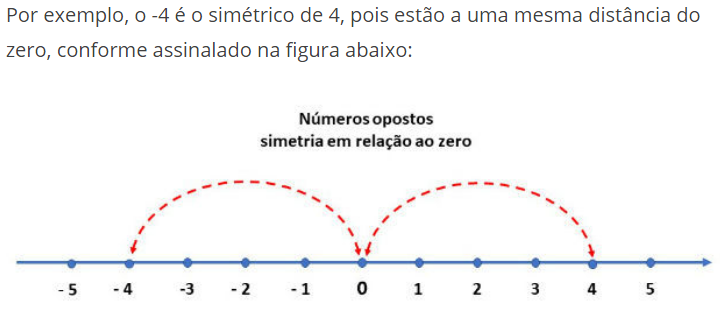
\includegraphics[height=30mm]{assets/Reta Conjunto dos Inteiros.png}
    \end{tabular}


    \begin{tabular}{@{}c@{}}
        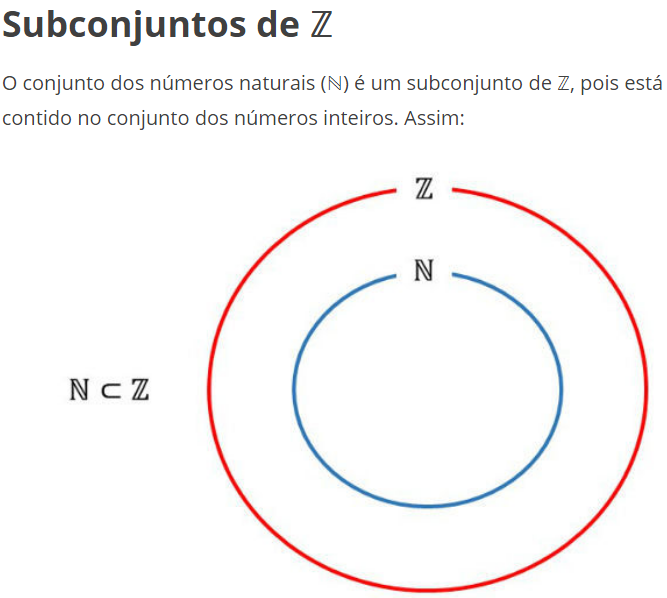
\includegraphics[height=65mm]{assets/Conjunto dos Inteiros Mais os Naturais Nele Contido.png}
    \end{tabular}

    Destaquemos agora alguns subconjuntos dos Inteiros $*\mathbb{Z}$:

    \begin{enumerate}

        \item $\mathbb{Z}$: É o subconjunto dos números inteiros, com exceção do zero. $\mathbb{Z}^* $ = {..., -3,-2,-1, 1, 2, 3, 4, ...}

        \item $\mathbb{Z}_*$: São os números inteiros não-negativos, ou seja $\mathbb{Z}_+ $ = {0, 1, 2, 3, 4, ...}

        \item $\mathbb{Z}_-$: É o subconjunto dos números inteiros não-positivos, ou seja $\mathbb{Z}_- $ = {..., -4,-3,-2,-1, 0}

        \item $\mathbb{Z}^*_+$: É o subconjunto dos números inteiros, com exceção dos negativos e do zero.$mathbb{Z}^*-+ $ = {1,2,3,4, 5...}

        \item $\mathbb{Z}^*_-$: São os números inteiros, com exceção dos positivos e do zero, ou seja $\mathbb{Z}^*_- $= {..., -4,-3,-2,-1}

    \end{enumerate}

    \subsection{Conjunto dos Números Racionais - $\mathbb{Q}$}

    O conjunto $\mathbb{Q} $ dos números racionais é formado por todos aqueles números que podem ser expressos na forma de fração $\dfrac{a}{b}$, em que "a"\ e "b"\ são números inteiros e "b"\ é diferente de 0.

    \textbf{Nota:} Em uma fração:

    O \textbf{numerador} é o número acima e o \textbf{denominador} é o número abaixo da mesma.

    $ \dfrac{A}{B} $, onde\\

    $\, \, \, \, \, \, \, \, \, \, \, \, \, \, \, \, \, \,A \, \, $ é o \textbf{Numerador} $\, \, \, \, \, \, \, \, \, \, \, \, \, $ e\\

    $\, \, \, \, \, \, \, \, \, \, \, \, \, \, \, \, \, \,B \, \, $ é o \textbf{Denominador}.\\

    Conhecido também como o conjunto das frações equivalentes à fração irredutível, ex: $\dfrac{3}{4}$.\\

    Um conjunto de frações equivalentes representa um único número racional.

    Cada fração do conjunto é um representante do número racional, e a fração irredutível com denominador positivo é o representante canônico.

    Assim, o número racional $\dfrac{2}{3} $ é formado pela fração $\dfrac{2}{3} $Fração e todas as suas equivalentes:

    Ao calcular a expressão decimal de um número racional, dividindo o numerador pelo denominador, obtêm-se números inteiros ou decimais.

    Os números decimais podem ter:

    Um número finito de algarismos, número decimal exato, se os únicos divisores do denominador forem 2 ou 5.

    Um número infinito de algarismos, que se repetem de forma periódica a partir da vírgula, decimal periódico simples, se 2 ou 5 forem divisores do denominador;

    A partir do algarismo dos décimos, centésimos…, decimal periódico composto, se entre os divisores do denominador estiver o 2 ou o 5 e houver, além desses, outros divisores.

    Reciprocamente, qualquer número decimal exato ou periódico pode ser expresso na forma de fração.

    Numeros Racionais
    Exemplo:
    Expressar na forma de fração os seguintes números decimais:

    \begin{enumerate}

        \item $1,92 \ = \ \dfrac{192}{100}$\\

        \item $1,\overline{73} \ = \ \dfrac{1,73 - 1}{99} \ = \ \dfrac{172}{99}$\\

        \item $1,7\overline{3} \ = \  \dfrac{173 - 17}{90} \ = \ $ \\ $ \dfrac{156}{90} \ = \ \dfrac{26}{15}$\\

        \item $1,07\overline{3} \ = \ \dfrac{1073 - 107}{900}\ = $\\ $ \ \dfrac{966}{900} \ = \ \dfrac{161}{150}$

    \end{enumerate}

    Representação canônica de um número racional.

    Dada uma fração, existem infinitas frações equivalentes a ela.

    Ex:

    $ \left\lbrace \dots \dfrac{-8}{-9}, \dfrac{-4}{-6}, \dfrac{-2}{-3}, \dfrac{2}{3}, \dfrac{4}{6},\dfrac{8}{9} \dots \right\rbrace $\\

    É o conjunto das frações equivalentes à fração irredutível.

    Um conjunto de frações equivalentes representa um único número racional, conforme os exemplos acima.

    Cada fração do conjunto é um representante do número racional, e a fração irredutível com denominador positivo é o representante canônico.

    Assim, o número racional Fração é formado pela Fração e todas as suas equivalentes:

    Todas elas são representantes do número racional $\dfrac{2}{3} $.

    Portanto, $ \dfrac{2}{3} $ é o representante canônico.\\

    \subsection{Conjunto dos Números Irracionais - $\mathbb{I}$}

    O conjunto $\mathbb{I}$ dos números irracionais é formado pelos números que não podem ser expressos em forma de fração. São números cuja expressão decimal tem um número infinito de algarismos que não se repetem de forma periódica.

    Existem infinitos números irracionais, e geralmente as raízes não exatas são também números irracionais, conforme abaixo:

    Exs:  $\sqrt{3}, \sqrt{7}, \sqrt{13}, \sqrt{2,737}, \sqrt{2}, \Pi$

    Estes números podem ser resultados de equações, cálculos de área, etc.

    \subsection{Conjunto dos Números Reais - $\mathbb{R}$}

    Os Números Reais $\mathbb{R}$, é o conjunto que contém todo o conjuntos dos números Naturais $\mathbb{N}$, números Inteiros $\mathbb{I}$, dos números Racionais $\mathbb{Q}$ e dos números Irracionais $\mathbb{I}$, conforme figura abaixo:

    \begin{tabular}{@{}c@{}}
        \includegraphics[height=60mm]{assets/Números Reais.png}
    \end{tabular}

    Fonte: Internet

    Pela figura acima, podemos fazer a seguinte observação:

    $\Rightarrow$ O conjunto dos números Naturais $\mathbb{N}$ está contido no conjunto dos número inteiros $\mathbb{Z}$, que está contido no conjunto dos números Racionais $\mathbb{Q}$, que também está contido no conjunto dos Números Reais $\mathbb{R}$, que por sua vez contém o conjunto dos números Irracionais $\mathbb{I}$, todavia, este último, não contém nenhum dos demais conjuntos, por esta razão, fica separado dos demais, mas dentro do conjunto dos números Reais $\mathbb{R}$.

    Todo número real tem um único ponto correspondente na reta e qualquer ponto da reta tem um único número real correspondente.

    Dizemos de forma intuitiva que o conjunto dos números Reais $\mathbb{R}$ é formado por todos os números que podem ser representados na reta numérica. Para representar subconjuntos ou intervalos da reta real usamos a representação geométrica ou uma notação própria utilizada no estudo dos conjuntos, conforme alguns exemplos na figura abaixo:

    \begin{tabular}{@{}c@{}}
        \includegraphics[height=37mm]{assets/Reta Numérica.png}
    \end{tabular}

    Fonte: 	https://www.infoescola.com/
    matematica/numeros-reais/\\

    \subsection{Conjunto dos Números Complexos - $\mathbb{C}$}

    O conjunto dos números Complexos compreedem os números compostos por uma parte real e outra imaginária.

    Representam o conjunto de todos os pares ordenados (x, y), cujos elementos pertencem ao conjunto dos números reais $\mathbb{C}$.

    É indicado por $\mathbb{C}$ e definido pelas operações seguintes:

    \textbf{Igualdade:} (a, b) = (c, d) $\Longleftrightarrow$ a = c e b = d

    \textbf{Adição:} (a, b) + (c, d) = (a + b + c + d)

    \textbf{Multiplicação:} (a, b) . (c, d) = (ac – bd, ad + bc)

    A unidade imaginária é indicada pela letra " i " e representa o par ordenado (0,1), assim,

    $i \cdot i = -1 \leftrightarrow i^2 = -1$

    Dessa forma, i é a raiz quadrada de -1, por isso i é chamado de \textbf{unidade imaginária}, pois não existe raiz quadrada de número negativo.

    Vejamos as potências de i:

    $ i^0 = 1$
    $ i^1 = i $
    $ i^2 = -1$
    $ i^3 = -i $
    $ i^4 = 1$
    $ i^5 = i$
    $ i^6 = -1$
    $ i^7 = -i$
    $ i^8 = 1 \dots$

    Observe que sempre vai repetindo os resultados de 0 a 4. Então, pegamos o expoente e dividimos por 4, e pegamos o resto, assim, fica fácil de fazer qualquer potenciação de i.

    Os números Complexos $\mathbb{C}$ são representados na forma algébrica da seguinte maneira:

    z = x + yi

    Onde x e y são números reais e " i " a parte imaginária.

    \textbf{Conjugado de um Número Complexo}

    O conjugado de um número complexo é indicado por z, definido por \textbf{z = a – bi}. Assim, troca-se o sinal de sua parte imaginária.

    Então, se \textbf{z = a + bi}, logo, o seu conjugado é \textbf{$\overline{z}$ = a – bi}.

    Quando multiplicamos um número complexo pelo seu conjugado, o resultado será um número real $\mathbb{R}$.

    Ex:

    $ (5 + 3i) \cdot (5 - 3i) $

    $ 5^2 - 3i + 3i - (3i)^2 \, Obs. (i^2 = -1)$

    $ 25 - [(9) \cdot (-1)] $

    $ 25 - (-9)$

    $ 25 + 9 $

    $ 34 \in \mathbb{R}$

    \textbf{Adição de Números Complexos:}

    $ z_1 + z_2 = ( a + c, b + d)$

    Ou algebricamente:

    $(a + bi) + (c + di) = (a + c) + i(b + d)$

    Ex:

    $(3 + 2i) + (-4 + 5i)$

    $(3 - 4) + i(2 + 5)$

    $ -1 + 7i$

    \textbf{Subtração de Números Complexos}

    $z_1 - z_2 = (a -c), b -d)$

    Ou algebricamente:

    $(a + bi) - (c + di) = (a - c) + i(b - d)$

    Ex:

    $(3 - 2i) - (-4 - 5i)$

    $(3 + 4) + i(-2 - 5)$

    $ 7 - 7i$

    \textbf{Multiplicação de Números Complexos:}

    $ (a, b) \cdot (c, d) = (ac - bd, ad + bc) $

    Ou algebricamente:

    $ (a + bi) \cdot (c + di) = ac +adi + bci +bdi^2 \longrightarrow (i^2 = -1) $

    $ (a + bi) \cdot (c + di) = ac + adi +bci - bd $

    $ (a +bi) \cdot (c + di) = (ac - bd) + i(ad + bc) $

    Ex:

    $ (4 + 3i) \cdot (2 - 5i) $

    $ 8 -20i + 6i - 15i^2 $

    $ 8 - 14i + 15 $

    $ 23 - 14i $

    \textbf{Divisão de Números Complexos:}

    Ao dividirmos dois números complexos devemos escrevê-los em forma de fração e multiplicarmos o numerador e o denominador pelo conjugado do denominador, veja como:

    $ z_1 \div z_2  =  \dfrac{z_1}{z_2} \cdot \dfrac{\overline{z_2}}{\overline{z_2}} $\\

    Exemplo: Sejam $ z_1 = 1 + i  \, e \,  z_2 = 1 +2i $

    $ \dfrac{z_1}{z_2} = \dfrac{1 + i}{1 + 2i} \cdot \dfrac{(1 - 2i)}{(1 - 2i)} = $\\

    $ \dfrac{1 - 2i + i -2i^2}{1 - 4i^2} = \dfrac{1 - i + 2}{1 +4} \dfrac{3 - i}{5} $\\

    Portanto: $ z_1 \cdot z_2 = \dfrac{3}{5} - \dfrac{i}{5} $\\

    De uma forma geral podemos demonstrar a divisão de dois números complexos por:

    Dado z1 = a + bi e z2 = c + di a divisão de z1 : z2 será:

    $ \dfrac{z_1}{z_2} = \dfrac{(a + bi)}{(c + di)} \cdot \dfrac{(c - di)}{c - di)} = $ \\

    $ \dfrac{ac - adi + cbi - bdi^2}{c^2 - d^2i^2} = $\\

    $ \dfrac{z_1}{z_2}= \dfrac{ac + bd + cbi - adi}{c^2 + d^2}= $\\

    $ \dfrac{ac + bd + (cb - ad)i}{c^2 + d^2} $\\

    Portanto: $ \, \, z_1 \div z_2= $

    $\dfrac{ac + bd + (cb - ad)i}{c^2 + d^2}$

    \textbf{Fórmula da divisão de números complexos.}

    \textbf{Propriedades:}

    $\Rightarrow |z| = |\overline{z}| $ O módulo do conjugado de um número complexo será o mesmo módulo do número;

    $\Rightarrow z \cdot \overline{z} = z^2 $ O produto de um número complexo pelo seu conjugado é o quadrado do módulo desse número, portanto, um número Real $\mathbb{R}.$

    $\Rightarrow z + \overline{z} = 2 x \in \mathbb{R} $ A soma de um número complexo ao seu conjugado resulta no dobro da parte real do número;

    $\Rightarrow z - \overline{z} = 2yi \in \mathbb{C} $ A subtração de um número complexo com seu conjugado resulta no dobro da parte imaginária desse número.


    \section*{Operações de Conjuntos}

    Os conjuntos são representados por letras maiúsculas, A, B, C, D...

    Caso todos os elementos de A também pertençam ao conjunto B, fica evidente que A é subconjunto do conjunto B, ou que A está contido em B, ou ainda que A é parte de B. A representação em forma de diagrama de um caso como esse é apresentada na imagem abaixo:

    \begin{tabular}{@{}c@{}}
        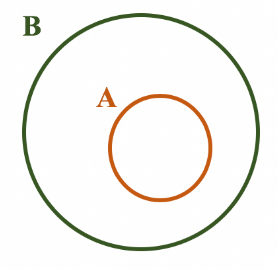
\includegraphics[height=60mm]{assets/Conjunto Contido.png}
    \end{tabular}

    Fonte: Autor\\

    Caso nenhum elemento de A também pertença ao conjunto B, e claro, nenhum elemento de B também pertença ao conjunto A, pode se dizer que A e B são conjuntos disjuntos. Nesse caso, o diagrama de cada um dos conjuntos é representado da seguinte forma:\\

    \begin{tabular}{@{}c@{}}
        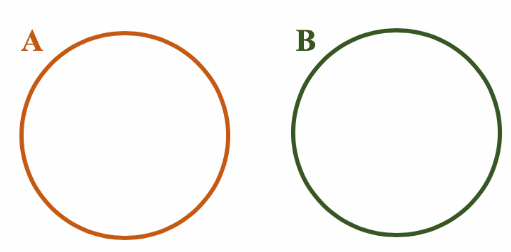
\includegraphics[height=35mm]{assets/Conjunto Disjunto.png}
    \end{tabular}

    Fonte: Autor\\

    Se apenas alguns elementos do conjunto A também pertençam ao conjunto B e vice-versa. Nesse caso, é comum entrelaçar os diagramas, para que os elementos comuns a ambos os conjuntos se localizem na região comum aos dois diagramas, como mostra a imagem:\\

    \begin{tabular}{@{}c@{}}
        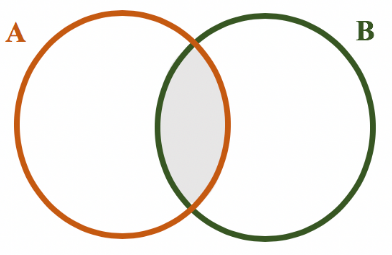
\includegraphics[height=40mm]{assets/Conjunto Intersecção.png}
    \end{tabular}

    Fonte: Autor\\

    \subsection{União entre Conjuntos}

    União entre dois ou mais conjuntos será determinado por um novo conjunto que se constituirá de elementos de pelo menos 1 dos conjutos, ou seja, somar os elementos de todos os conjuntos em um único conjunto, sem repetir, caso algum dos conjuntos tenha o mesmo ítem ou número.

    Para representar a união usamos o símbolo: $ \mathbf{ \cup } $.

    Definição:

    $A\cup B=\{x|x\in A\lor x\in B\}$

    \begin{tabular}{@{}c@{}}
        \includegraphics[height=50mm]{assets/União Conjuntos.png}
    \end{tabular}

    Fonte: Autor.

    Sejam os conjuntos A = {h, a, s, e, t} e B = {a, e, i, o, u}, represente o conjunto união (A U B).

    Para encontrar o conjunto união basta juntar os elementos dos dois conjuntos dados.

    Temos de ter o cuidado de incluir os elementos que se repetem nos dois conjuntos uma única vez.

    Assim, o conjunto união será:

    A U B = {h, a, s, e, t, i, o, u}

    \subsection{Interseção entre Conjuntos}

    A interseção de um conjunto A com um conjunto B, pode ser dita como o conjunto formado pelos elementos que pertencem a A e a B.

    Para representar a interseção usamo o símbolo: $ \cap $.

    Definição:

    $\displaystyle A\cap B=\{x|x\in A\land x\in B\}$

    Interseção entre conjuntos\\

    \begin{tabular}{@{}c@{}}
        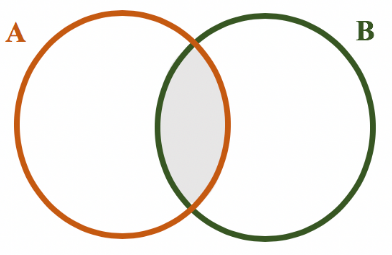
\includegraphics[height=45mm]{assets/Conjunto Intersecção.png}
    \end{tabular}

    Fonte: Autor

    Observação: Quando os conjuntos não apresentam elementos comuns entre si, dizemos que a interseção é um conjunto vazio ($\emptyset$).

    Nesse caso, esses conjuntos são chamados de disjuntos:

    A $ \cap $ B = $\emptyset$.

    \subsection{Diferença entre Conjuntos}

    Seja o Conjunto A = $\{{ 0, 1, 2, 3, 4 }\}$ e B = $\{ 4, 5, 6 \}$, a diferença entre esses dois conjuntos (A - B), é um outro conjunto ao qual chamamos de Conjunto Diferença.

    Neste caso a operação se dá da seguinte forma: Os elementos do Conjunto (A) Menos os Elementos do Conjunto (B):

    Conjunto Diferença (C) = $\{ 0, 1, 2, 3 \}$

    Quando fazemos a diferença entre conjuntos, eliminamos os elementos que são comuns entre eles e mantemos os outros elementos do conjunto que inicia a operação, no caso, o conjunto A, pois temos (A - B).

    Se tivéssemos (B - A), o conjunto resultante que chamamos de conjunto diferença, ficaria assim:

    B = $\{ 5, 6 \}$

    \subsection{Conjunto Complementar}

    O conjunto complementar está relacionado com a diferença entre dois ou mais conjuntos, todavia, é necessário que o conjunto B tenha todos os seus elementos representados no conjunto A para que se verifique o complementar de A em relação a B.

    Seja $ A =\{0,1, 2, 3, 4, 5, 6, 7, 8, 9\} $ e $ B = \{ 2, 4, 6, 8\} $

    O Complementar do conjunto A em relação ao conjunto B é:

    $ C_A^B = \{0, 1, 3, 5, 7, 9 \} $.

    Lê-se da seguinte maneira: complementar de (B) em relação a (A).

    \textbf{Importante:} Os elementos do conjunto (B) devem estar contidos no conjunto (A).

    Se desejásemos saber o complementar de um conjunto (E) em relação ao conjunto (A), este conjunto (E), obrigatoriamente, deve estar contido no conjunto (A).

    Caso o conjunto (E) fosse: E = $\{9, 4, 1\}$, o complemetar de (E) em relação a (A), seria:

    $ C_A^E = \{ 0, 2, 3, 5, 6, 7, 8\}$

    Caso o conjunto (E) não estivesse contido no conjunto (A), não seria possível determinar o complementar do conjunto (E) em relação ao conjunto (A).

    \subsection{Símbolos usados com conjuntos}

    Os símbolos geralmente usados com conjuntos são os seguintes:\\

    $\cup$ União

    $\cap$ Interseção

    $\supset$ Contém

    $\not \supset$ Não Contém

    $\subset$ Está Contido

    $\not \subset$ Não está Contido

    $\in$ Pertence

    $\not \in$ Não Pertence

    $\ni$ Existe

    $\not \ni$ Não Existe

    $\ni !$ Existe um Único.

    $\forall $ Para Todo.\\

    Existem muitos outros símbolos, porém estes são os mais comuns e os que precisaremos.

    %\pagebreak

    \subsection{Exercícios}

    \begin{enumerate}

        \item (Uece – 2016) Dados os números racionais $ \dfrac{3}{7},\, \dfrac{5}{6},\, \dfrac{4}{9},\, \dfrac{3}{5}$, a divisão do menor deles pelo maior é igual a:

              a) $\frac{27}{28} \ \ \ $ b) $\frac{18}{25} \ \ \ $ c) $\frac{18}{35} \ \ \ $ d) $\frac{20}{27}$

        \item (Ueg – 2015) Se colocarmos os números reais $ - \sqrt{5},\, 1,\, - \dfrac{3}{5}\, $ e $\, \dfrac{3}{8}$ em ordem decrescente, teremos a sequência:

              \begin{enumerate}

                  \item $\frac{3}{8},\, 1,\,- \frac{3}{5},\, -\sqrt{5}$
                  \item $\frac{3}{8},\, 1,\,-\sqrt{5},\, - \frac{3}{5}$
                  \item $1,\, \frac{3}{8},\, - \frac{3}{5},\, -\sqrt{5},$
                  \item $1,\, \frac{3}{8},\, 1,\, -\sqrt{5},\, - \frac{3}{5}$

              \end{enumerate}

        \item (Upf – 2015) Dividindo 2 por 7, o 100° algarismo da expansão decimal que aparece após a vírgula é:

              a) $ 1 \ \ $ b) $ 2 \ \ $ c) $ 5 \ \ $ d) $ 7 \ \ $ e) $ 8 \ \ $

        \item (Uece – 2015) Se a soma e o produto de dois números são, respectivamente, dois e cinco, podemos afirmar corretamente que:

              \begin{enumerate}

                  \item  os dois números são racionais.
                  \item  os dois números são irracionais
                  \item  um dos números é racional e o outro é irracional.
                  \item  os dois números são complexos não reais.

              \end{enumerate}

        \item (Pucrs – 2015) Em nossos trabalhos com matemática, mantemos um contato permanente com o conjunto $ mathbb{R} $ dos números reais, que possui, como subconjuntos, o conjunto $ mathbb{N} $ dos números naturais, o conjunto $ mathbb{Z} $ dos números inteiros, o $ mathbb{Q} $ dos números racionais e o dos números irracionais $ mathbb{I} $. O conjunto dos números reais também pode ser identificado por:

              \begin{enumerate}

                  \item $ \mathbb{R} \cup \mathbb{Z} $
                  \item $ \mathbb{N} \cup \mathbb{Q} $
                  \item $ \mathbb{Z} \cup \mathbb{Q} $
                  \item $ \mathbb{Z} \cup \mathbb{I} $
                  \item $ \mathbb{Q} \cup \mathbb{I} $

              \end{enumerate}

        \item (Enem – 2015) Deseja-se comprar lentes para óculos. As lentes devem ter espessuras mais próximas possíveis da medida 3 mm. No estoque de uma loja, há lentes de espessuras: 3,10 mm; 3,021 mm; 2,96 mm; 2,099 mm e 3,07 mm.
              Se as lentes forem adquiridas nessa loja, a espessura escolhida será, em milímetros, de:

              \begin{enumerate}

                  \item 2,099
                  \item 2,96
                  \item 3,021
                  \item 3,07
                  \item 3,10

              \end{enumerate}

        \item (Enem PPL – 2014) Um clube de futebol, abriu inscrições para novos jogadores. Inscreveram-se 48 candidatos. Para realizar uma boa seleção, deverão ser escolhidos os que cumpram algumas exigências: os jogadores deverão ter mais de 14 anos, estatura igual ou superior à mínima exigida e bom preparo físico. Entre os candidatos, $\dfrac{7}{8}$ têm mais de 14 anos e foram pré-selecionados. Dos pré-selecionados $\dfrac{1}{2}$ têm estatura igual ou superior à mínima exigida e, destes, $\dfrac{2}{3}$ têm bom preparo físico. A quantidade de candidatos selecionados pelo clube de futebol foi de:

              a) $12 \ \ $ b) $14 \ \ $ c) $16 \ \ $ d) $32 \ \ \ \ $ e) $42 \ \ $

        \item (Ifce – 2014) Considere os seguintes números reais $\dfrac{23}{24},\, \dfrac{7}{8},\, \dfrac{47}{48},\, 1, \dfrac{11}{12},\, \dfrac{4}{3},\, \dfrac{11}{8} $. Colocando-se esses números em ordem crescente, o menor e o maior deles são, respectivamente:

              \begin{enumerate}

                  \item $ \frac{23}{24}$ ? $ 1 $
                  \item $ \frac{11}{12}$ ? $ \frac{4}{3} $
                  \item $ \frac{7}{8}$ ? $ \frac{4}{3} $
                  \item $ \frac{7}{8}$ ? $ \frac{11}{8} $
                  \item $ \frac{47}{48}$ ? $ \frac{4}{3} $

              \end{enumerate}

        \item (Ueg – 2016) Dados os conjuntos ? = {? $\in \mathbb{R}|-2 <  ?  \leq 4\} e ? = \{? \in \mathbb{R}|$ ? > 0}, a intersecção entre eles é dada pelo conjunto:

              \begin{enumerate}

                  \item {? $\in \mathbb{R}$|0 < ? $\leq$ 4}
                  \item {? $\in \mathbb{R}$|? > 0}
                  \item {? $\in \mathbb{R}$|? > $ -2 $}
                  \item {? $\in \mathbb{R}$|? $\geq$ 4}

              \end{enumerate}

        \item (Ifpe – 2016) Em uma cooperativa de agricultores do município de Vitória de Santo Antão, foi realizada uma consulta em relação ao cultivo de cana-de-açucar e do algodão. Constatou-se que 125 associados cultivavam a cana-de-açucar, 85 cultivavam o algodão e 45 cultivavam ambos. Sabendo que todos os cooperativados cultivavam pelo menos uma dessas duas culturas. Qual é o número de agricultores da cooperativa?

              a) $210 \ \ $ b) $255 \ \ $ c) $165 \ \ \ \ \ \ \ \ \ \ $ d) $125 \ \ $ e) $45 \ \ $

        \item (Uepa – 2015) De acordo com a reportagem da Revista Veja (edição 2341), é possível fazer gratuitamente curso de graduação pela Internet. Dentre os ofertados temos os cursos de Administração (bacharelado), Sistemas de Computação (Tecnólogo) e Pedagogia (licenciatura). Uma pesquisa realizada com 1.800 jovens brasileiros sobre quais dos cursos ofertados gostariam de fazer, constatou-se que 800 optaram pelo curso de Administração; 600 optaram pelo curso de Sistemas de Computação; 500 optaram pelo curso de Pedagogia; 300 afirmaram que fariam Administração e Sistemas de Computação; 250 fariam Administração e Pedagogia; 150 fariam Sistemas de Computação e Pedagogia e 100 dos jovens entrevistados afirmaram que fariam os três cursos. Considerando os resultados dessa pesquisa, o número de jovens que não fariam nenhum dos cursos elencados é:

              a) $150 \ \ $ b) $250 \ \ $ c) $350 \ \ \ \ \ \ \ \ \ \ $ d) $400 \ \ $ e) $500 \ \ $

        \item (Fuvest) No alto de uma torre de uma emissora de televisão duas luzes “piscam” com freqüências diferentes. A primeira “pisca” 15 vezes por minuto e a segunda “pisca” 10 vezes por minuto. Se num certo instante as luzes piscam simultaneamente, após quantos segundos elas voltarão a piscar simultaneamente?

              a) $12 \ \ \ $ b) $10 \ \ \ $ c) $20 \ \ \ $ d) $15 \ \ \ \ $ e) $30 \ \ $

    \end{enumerate}

    \section*{Porcentagem e Juros Simples}

    Para trabalharmos com porcentagem e juros simples, que é o foco deste capítulo, precisamos relembrar como funciona a Regra de Três Simples, pois este conhecimento, muito nos auxiliará neste tópico.

    \subsection{Regra de Três Simples}

    A regra de três é um método que utilizamos para encontrar valores desconhecidos quando estamos trabalhando com grandezas direta ou inversamente proporcionais.

    Regra de três simples é um processo prático para resolver problemas que envolvam quatro valores dos quais conhecemos três deles. Devemos, portanto, determinar um valor a partir dos três já conhecidos.

    Esse método de resolução tem bastante aplicação não só na matemática, como na física, química e em situações constantes do dia a dia. O trabalho com grandezas é fundamental em várias áreas do conhecimento, e, na regra de três, é importante conseguir-se identificar grandezas que se relacionam de forma direta e grandezas que se relacionam de forma inversa.

    A comparação entre duas grandezas é bastante comum e necessária no cotidiano, e quando comparamos e verificamos sua proporção, podemos separá-las em dois casos importantes: grandezas diretamente proporcionais ou grandezas inversamente proporcionais.

    \textbf{Diretamente proporcionais:} à medida que uma dessas grandezas aumenta, a outra também aumenta e na mesma proporção. Um exemplo de grandeza diretamente proporcional seria caminhar em relação ao tempo, quanto mais se caminha, mais tempo gasta, quanto menos se caminha, menos tempo se gasta, isso para uma velocidade constante de caminhar.

    \textbf{Inversamente proporcionais:} à medida que uma dessas grandezas aumenta, a outra grandeza diminui na mesma proporção. Um exemplo de grandeza inversamente proporcional seria velocidade em relação ao tempo, quanto maior a velocidade, menos o tempo para percorrer a mesma distância.

    Passos utilizados numa regra de três simples:

    \textbf{1º)} Construir uma tabela, agrupando as grandezas da mesma espécie em colunas e mantendo na mesma linha as grandezas de espécies diferentes em correspondência.

    \textbf{2º)} Identificar se as grandezas são diretamente ou inversamente proporcionais.

    \textbf{3º)} Montar a proporção e resolver a equação.

    \textbf{Exemplo:} Uma fábrica com 7 máquinas, produz 1253 peças de um determinado produto. Quantas peças produzirá se utilizar 9 máquinas?

    Se o número de máquinas aumenta, a produção aumenta, logo, são grandezas diretamente proporcionais.

    7 máquinas produz 1253 peças, quantas peças produzirão 9 máquinas?

    7  ---   1253
    9  ---      X

    Basta então multiplicarmos de forma cruzada, da seguinte forma:

    7X = 9$\cdot$ 1253  \\

    X = $\dfrac{11277}{7}$\\

    X = 1.611  ==> Serão produzidas 1611 peças.\\

    \textbf{Exemplo 2:} Para deslocar-se de uma cidade para a outra, a uma velocidade média de 80 km/h, leva-se exatamente 2 horas e 55 minutos. Qual seria o tempo gasto se a velocidade fosse de 100 km/h:

    Grandeza inversamente proporcional. Velocidade aumenta, tempo diminui.

    80  ---  175 minutos (aqui você precisa transformar o tempo em minutos)
    100 --    X

    Logo:   100X = 80$\cdot$175    ==>  X = $\dfrac{14000}{100}$    ==>   X = 140\\

    140 minutos equivalem a duas horas e 20 minutos.

    \subsection{Exercícios de Regra de Três Simples}

    \begin{enumerate}

        \item (ENEM) Uma televisão pode ser posicionada de modo que se consiga enxergar os detalhes de uma imagem em alta definição. Considere que a distância ideal, com conforto visual, para se assistir à televisão de 32 polegadas
              é de 1,8 metro. Supunha que haja uma relação de proporcionalidade direta entre o tamanho da tela (medido
              em polegada) e a distância ideal. Considere que um espectador dispõe de uma televisão de 60 polegadas e que
              ele deseja se posicionar em frente a ela, com conforto visual.

              A distância da televisão, em metro, em que o espectador deve se posicionar para que tenha conforto visual é mais
              próxima de

              a) $0,33 \ \ $ b) $0,96 \ \ $ c) $157 \ \ \ \ \ \ \ \ \ \ $ d) $3,37 \ $ e) $3,60 \ \ $

        \item (ENEM) Nos shopping centers costumam existir parques com vários brinquedos e jogos. Os usuários
              colocam créditos em um cartão, que são descontados por cada período de tempo de uso dos jogos. Dependendo da
              pontuação da criança no jogo, ela recebe um certo número de tíquetes para trocar por produtos nas lojas dos parques.

              Suponha que o período de uso de um brinquedo em certo shopping custa R\$3,00 e que uma bicicleta custa 9200 tíquetes.

              Para uma criança que recebe 20 tíquetes por período de tempo que joga, o valor, em reais, gasto com créditos para
              obter a quantidade de tíquetes para trocar pela bicicleta é

              a) $153 \ \ \ \ \ $ b) $460 \ \ $ c) $1218 \ \ \ \ \ \ \ \ \ \ $ d) $1380 \ \ $ e) $3066 \ \ $

        \item (ENEM) Um confeiteiro deseja fazer um bolo cuja receita indica a utilização de açúcar e farinha de trigo em
              quantidades fornecidas em gramas. Ele sabe que uma determinada xícara utilizada para medir os ingredientes
              comporta 120 gramas de farinha de trigo e que três dessas xícaras de açúcar correspondem, em gramas, a quatro de
              farinha de trigo.

              Quantos gramas de açúcar cabem em uma dessas xícaras?

              a) $30 \ \ $ b) $40 \ \ $ c) $90 \ \ $ d) $160 \ \ $ e) $360 \ \ $

        \item Durante o ano de 2020, devido à pandemia de COVID-19, o mundo viu-se dependente da criação de uma vacina para imunizar a população. No Brasil não foi diferente, e a corrida por uma vacina eficaz só terminou no ano de 2021. A primeira delas foi a Coronavac, produzida pelo Instituto Butantan, que anunciou que a vacina possui 78\% de eficácia em casos leves. Isso significa que, se 100 pessoas forem vacinadas, 78 pessoas não terão sintoma algum e 22 pessoas terão sintomas leves.

              A partir desse anúncio, iniciou-se a campanha de imunização. Supondo-se que a cidade de Abadia de Goiás (próxima da capital Goiânia) tenha conseguido vacinar toda a sua população, que é de 8.950 habitantes, e considerando-se que toda ela tenha contato com o vírus e que essa proporção seja mantida, a quantidade de pessoas que terão sintomas leves nessa população será de:

              a) $6979 \ \ \ $ b) $6780 \ \ \ $ c) $2170 \ \ \ $ d) $1969 \ \ \ $ e) $1852 \ \ $

        \item A água é um dos recursos mais importantes para a manutenção da vida. Infelizmente, ela nem sempre é bem cuidada, o que tem gerado grandes contaminações de água potável em nossa sociedade. Um dos meios de contaminação é o descarte incorreto de óleo de cozinha, em que 1 litro de óleo contamina 25 mil litros de água que poderia ser potável. Preocupado com essa situação, o síndico de um condomínio resolveu colocar na área comum um tanque para descarte correto desse  óleo. Ao final do mês, ele coletou um total de 135,6 litros. Caso esse volume de óleo fosse jogado fora de maneira incorreta, o volume de água contaminada seria de:

              A) 3 milhões de litros

              B) 3,2 milhões de litros

              C) 3,4 milhões de litros

              D) 3,5 milhões de litros

              E) 4 milhões de litros

    \end{enumerate}

    \subsection*{Porcentagem}

    A porcentagem nada mais é do que uma multiplicação por uma fração de denominador cem, como veremos nos exemplos a seguir:

    $ 07\% = \frac{7}{100} = 0,07 $\\

    $ 23\% = \frac{23}{100} = 0,23 $\\

    $ 45\% = \frac{45}{100} = 0,43 $

    \textbf{Exemplo 1:} O salário de uma pessoa é de R\$ 1600,00 qual a quantia que ele receberá se o salário aumentar 15\% na sua promoção?

    15\% de 1600  =  $\dfrac{15}{100}*1600 = 240$

    Logo o salário será de (1600 + 240) = R\$1.840,00

    \textbf{Exemplo 2:} Em uma promoção relâmpago, sua compra de R\$ 120,00 ganhou um desconto de 20\%. Qual o valor que deverá pagar pela compra?

    20\% de 120  =  $\dfrac{20}{100} * 120 = 24$

    Logo, o valor a pagar é de (120 - 24) = R\$ 96,00

    \subsection{Juros Simples}

    \textbf{Terminologia básica:}

    \textbf{Capital} $(C)$: É o valor monetário inicial;

    \textbf{Juros} $(J)$: É o valor que incide sobre o capital ao longo do tempo, esse tempo no Brasil geralmente e expresso em meses.

    \textbf{Taxa} de Juros $(i)$: É o valor do juros numa determinada unidade de tempo (que pode ser mês, bimestre, trimestre, semestre, ano, etc.). Exemplo: Para i = 5\% ao mês: significa que a cada mês, você recebe 5 de juro para cada 100 de capital aplicado.

    \textbf{Taxas de juros proporcionais} – duas taxas  i1 e i2, relativas respectivamente aos períodos de tempos n1 e n2, são proporcionais se, supondo n1 e n2 expressos na mesma unidade, então, a taxa semestral de 12\% é proporcional à taxa mensal de 2\%, pois são proporcionais.

    \textbf{Taxas de juros equivalentes} – duas taxas i1 e i2 são equivalentes se, a despeito de estarem referidas a períodos de tempos diferentes, produzem montantes iguais, quando aplicadas ao mesmo capital e pelo mesmo prazo.

    \textbf{Montante} $(M)$: É a soma do capital com os juros auferidos:

    \textbf{M = C + J}

    O juros é igual ao capital vezes a taxa vezes o periodo (tempo) em que o dinheiro foi aplicado.

    Fórmula do Juros Simples (J):

    \textbf{J = C.i.n}

    Logo a fómula do montante substituindo o o juros pela fórmula do juros, fica:

    \textbf{M = C + C.i.n}, colocando o "C" em evidência, temos:

    \textbf{M = C (1 + i.n)}\\

    \textbf{Exemplos:}

    \begin{enumerate}

        \item O capital de R\$ 1.060,00 foi aplicado à taxa de juros simples de 3\% ao mês. Qual será o valor do montante, após 5 meses?		Montante = ?  ;  Capital = 1.060,00  ;  Taxa = 3\% ao mês  ;  Período = 5 meses.

              Juros = C.i.n  $\, \rightarrow \,  J = 1060 \cdot 3\% \cdot 5$

              Juros = R\$ 159,00

              Montante = C + J $ \, \rightarrow \, M = 1060 + 159 \, \rightarrow \, M = R\$1.219,00$

        \item Um capital de R\$ 600,00 aplicado à taxa de juros simples de 20\% ao ano, gerou  um  montante  de R\$ 1.080,00 após um certo tempo. Qual foi esse tempo?  $\, \, \, \, \, \, $  M = 1.080,00 ; C = 600 ; i = 20\% aa ; n = ?

              M = C + J $\, \, \rightarrow \, \,  1080 = 600 + J \, \, \rightarrow \, \, J = 1080 - 600 \, \, \rightarrow \, \, M= 480$

              $ J = C\cdot i \cdot n \, \, \rightarrow \, \, 480 = 600 \cdot 20\% \cdot n \, \, \rightarrow \, \, 480 = 120.n \, \, \rightarrow \, \, n = \dfrac{480}{120}\, \, \rightarrow \, \, n = 4 $ Logo o período é de 4 anos, pois a taxa foi dada em anos.

        \item A que taxa devemos aplicar o capital de R\$ 10.000,00, no regime de capitalização simples, para que após 7 meses, o montante seja de R\$ 12.100,00?  C = 10.000,00  ;  n = 7 meses  ;  M = 12.100,00 ;  i = ?

              M = C + J $\, \, \rightarrow \, \, 12100 = 10000 + J \, \, \rightarrow \, \, J = 12100 - 10000 \, \, \rightarrow \, \, J = 2100$\\

              $ J = C \cdot i \cdot n \, \, \rightarrow \, \,2100 = 10000 \cdot 7 \cdot i \, \, \rightarrow \, \, i = \dfrac{2100}{70000} \, \, \rightarrow \, \, i = 0,03 \, \, \rightarrow \, \, i = 3\% $. A taxa é de 3\% ao mês.

        \item Quanto renderá de juros a quantia de R\$ 1.000,00, aplicada no regime de capitalização simples, com taxa de 0,6\% ao mês, ao final de 4 anos e 6 meses? C = 1000 ; i = 0,6\% am ; n = 54 meses ( 4 x 12 + 6 = 54) ; J = ?

              $ J = C \cdot i \cdot n$.

              $ J = 1000 \cdot 0,6\% \cdot 54 $.

              $ J = R\$ 324,00 $.

              O valor renderá R\$ 324,00.

    \end{enumerate}

    \subsection{Exercícios Porcentagem e Juros Simples}

    \begin{enumerate}

        \item (ENEM) Uma ponte precisa ser dimensionada de forma que possa ter três pontos de sustentação. Sabe-se que a carga máxima suportada pela ponte será de 12 t. O ponto de sustentação central receberá 60% da carga da ponte, e o
              restante da carga será distribuído igualmente entre os outros dois pontos de sustentação. No caso de carga máxima, as cargas recebidas pelos três pontos de sustentação serão, respectivamente,

              a.1,8 t; 8,4 t; 1,8 t.

              b.3,0 t; 6,0 t; 3,0 t.

              c.2,4 t; 7,2 t; 2,4 t.

              d.3,6 t; 4,8 t; 3,6 t.

              e.4,2 t; 3,6 t; 4,2 t.

        \item (UERJ) O cálculo errado da gorjeta levou os dois amigos a pagarem uma conta de R\$ 58,00, quando o valor correto a ser pago deveria ser R\$ 18,00 + 10\% de R\$ 18,00. Se soubessem um pouquinho de aritmética, esses clientes
              poderiam ter economizado, em reais, a quantia de:

              a) $36,20 \ \ $ b) $38,20 \ \ $ c) $39,00 \ \ $ d) $48,20 $

        \item (ENEM) Um laboratório realiza exames em que é possível observar a taxa de glicose de uma pessoa. Os
              resultados são analisados de acordo com o quadro a seguir:

              \begin{tabular}{@{}c@{}}
                  \includegraphics[height=30mm]{assets/glicemia.png}
              \end{tabular}

              Um paciente fez um exame de glicose nesse laboratório e comprovou que estava com hiperglicemia. Sua taxa de
              glicose era de 300mg/dL. Seu médico prescreveu um tratamento em duas etapas. Na primeira etapa ele
              conseguiu reduzir sua taxa em 30\% e na segunda etapa em 10\%

              Ao calcular sua taxa de glicose após as duas reduções, o paciente verificou que estava na categoria de:

              a.hipoglicemia.

              b.normal.

              c.pré-diabetes.

              d.diabetes melito.

              e.hiperglicemia.


        \item (ENEM) O Brasil é um país com uma vantagem econômica clara no terreno dos recursos naturais, dispondo de uma das maiores áreas com vocação agrícola do mundo. Especialistas calculam que, dos 853 milhões de hectares do país, as cidades, as reservas indígenas e as áreas de preservação, incluindo florestas e mananciais, cubram por volta de 470 milhões de hectares. Aproximadamente 280 milhões se destinam à agropecuária, 200 milhões para pastagens e 80 milhões para a agricultura, somadas as lavouras anuais e as perenes, como o café e a fruticultura.

              FORTES, G. Recuperação de pastagens é alternativa para ampliar cultivos. Folha de S. Paulo, 30 out. 2011.

              De acordo com os dados apresentados, o percentual correspondente à área utilizada para agricultura em relação à área do território brasileiro é mais próximo de a.32,8\%.

              a) $28,6\% \ \ $ b) $10,7\% \ \ $ c) $ 9,4\% \ \ $ d) $ 8,0\% $

        \item (ENEM2AP) Uma fábrica de papel higiênico produz embalagens com quatro rolos de 30 m cada, cujo preço
              para o consumidor é R\$ 3,60. Uma nova embalagem com dez rolos de 50 m cada, de mesma largura, será lançada no
              mercado. O preço do produto na nova embalagem deve ser equivalente ao já produzido, mas, para incentivar as
              vendas, inicialmente o preço de venda terá um desconto de 10\%.

              Para que isso aconteça, o preço de venda da nova embalagem, em real, deve ser:

              a) $8,10 \ \ $ b) $9,00 \ \ $ c) $9,90 \ \ \ \ \ \ \ \ \ \ $ d) $13,50 \ \ $ e) $15 \ \ $

        \item (ENEM) Em uma empresa de móveis, um cliente encomenda um guarda-roupas nas dimensões 220 cm de
              altura, 120 cm de largura e 50 cm de profundidade. Alguns dias depois, o projetista, com o desenho elaborado na
              escala 1:8, entra em contato com o cliente para fazer sua apresentação. No momento da impressão, o profissional
              percebe que o desenho não caberia na folha de papel que costumava usar. Para resolver o problema, configurou a
              impressora para que a figura fosse reduzida em 20\%.

              A altura, a largura e a profundidade do desenho impresso para a apresentação serão, respectivamente:

              a.22,00 cm, 12,00 cm e 5,00 cm

              b.27,50 cm, 15,00 cm e 6,25 cm

              c.34,37 cm, 18,75 cm e 7,81cm

              d.35,20 cm, 19,20 cm e 8,00 cm

              e.44,00 cm, 24,00 cm e 10,00 cm

        \item (ENEM) O LIRAa, Levantamento Rápido de Índice de Infestação por Aedes aegypti, consiste num mapeamento da infestação do mosquito Aedes aegypti. O LIRAa é dado pelo percentual do número de imóveis com focos do mosquito, entre os escolhidos de uma região em avaliação. O serviço de vigilância sanitária de um município no mês de outubro do ano corrente, analisou o LIRAa de cinco bairros que apresentaram o maior índice de infestação no ano anterior. Os dados obtidos para cada bairro foram:

              I. 14 imóveis com focos de mosquiro em 400 imóveis no bairro;

              II. 6 imóveis com focos de mosquito em 500 imóveis no bairro;

              III. 13 imóveis com focos de mosquito em 520 imóveis no bairro;

              IV. 9 imóveis com focos de mosquito em 360 imóveis no bairro;

              V. 15 imóveis com focos de mosquito em 500 imóveis no bairro;

              O setor de dedetização do município definiu que o direcionamento das ações de controle iniciarão pelo bairro
              que apresentou o maior índice do LIRAa.

              As ações de controle iniciarão pelo bairro:

              a) $ I \ \ $ b) $ II \ \ $ c) $III \ \ $ d) $ IV \ \ $ e) $ V \ \ $

        \item (ENEM) Uma organização não governamental divulgou um levantamento de dados realizado em algumas cidades
              brasileiras sobre saneamento básico. Os resultados indicam que somente 36\% do esgoto gerado nessas cidades é tratado, o que mostra que 8 bilhões de litros de esgoto sem nenhum tratamento são lançados todos os dias nas águas. Uma campanha para melhorar o saneamento básico nessas cidades tem como meta a redução da quantidade de esgoto lançado nas águas diariamente, sem tratamento, para 4 bilhões de litros nos próximos meses.

              Se o volume de esgoto gerado permanecer o mesmo e a meta dessa campanha se concretizar, o percentual de esgoto tratado passará a ser:

              a) $72\% \ \ $ b) $68\% \ \ $ c) $64\% \ \ \ \ \ \ \ \ \ \ $ d) $54\% \ \ $ e) $18\% \ \ $

        \item (ENEM2aAP) Em certa loja de roupas, o lucro na venda de uma camiseta é de 25\% do preço de custo da camiseta pago pela loja, Já o lucro na venda de uma bermuda é de 30\% do preço de custo da bermuda, e na venda de uma calça o lucro é de 20\% sobre o preço de custo da calça. Um cliente comprou nessa loja duas camisetas, cujo preço de custo foi R\$ 40,00 cada uma, uma bermuda que teve preço de custo de R\$ 60,00 e duas calças, ambas com mesmo
              preço de custo. Sabe-se que, com essa compra, o cliente proporcionou um lucro de R\$ 78,00 para a loja.

              Considerando essas informações, qual foi o preço de custo, em real, pago por uma calça?

              a) $90 \ \ \ \ \ \ $ b) $100 \ \ \ \ \ $ c) $125 \ \ \ \ \ \ \ \ \ \ \ \ \ $ d) $195 \ \ $ e) $200 \ \ $

    \end{enumerate}

    \section*{Princípio de Contagem}

    \textbf{Princípio Fundamental da Contagem:} é o  conceito principal ensinado na análise combinatória. A partir dele que se desenvolveram os demais conceitos dessa área e as fórmulas de fatorial, combinação, arranjo, permutação. Entender esse princípio é essencial para compreender situações que envolvem contagem.

    Esse princípio diz que, se eu preciso tomar mais de uma decisão e cada uma delas pode ser tomada de x, y, z (diversas) maneiras, para sabermos a quantidade de formas que essas decisões podem ser tomadas simultaneamente, basta calcular o produto dessas possibilidades.

    O que é o princípio fundamental da contagem?

    O princípio fundamental da contagem é \textbf{uma técnica para calcularmos de quantas maneiras decisões podem combinar-se}. Se uma decisão pode ser tomada de "n" maneiras e outra decisão pode ser tomada de "m" maneiras, o número de maneiras que essas decisões podem ser tomadas simultaneamente é calculado pelo produto de "n · m".

    Analisar todas as combinações possíveis sem utilizar o princípio fundamental da contagem pode ser bastante trabalhoso, o que faz com que a fórmula seja muito eficiente.

    \textbf{Ex.:} Em um restaurante, é oferecido o famoso prato feito. Todos os pratos possuem arroz, e o cliente pode escolher uma combinação entre 3 possibilidades de carne (bovina, de frango e vegetariana), 2 tipos de feijão (caldo ou tropeiro) e 2 tipos de bebida (suco ou refrigerante). De quantas maneiras distintas um cliente pode fazer o pedido?

    \begin{tabular}{@{}c@{}}
        \includegraphics[height=55mm]{assets/combinatória.png}
    \end{tabular}
    Fonte: https://brasilescola.uol.com. br/matematica/fatorial-principio- fundamental-da-contagem.htm

    Observe que há 12 possibilidades para escolher, mas seria possível chegar a esse número realizando a multiplicação das possibilidades por meio do princípio fundamental da contagem, logo o número de combinações de pratos possíveis poderia ser calculado por:

    2 · 3 · 2 = 12.

    Perceba que, quando meu interesse é saber somente o total de possibilidades, realizar a multiplicação é muito mais rápido do que construir qualquer esquema para analisar, o que pode ser bastante trabalhoso, caso haja mais e mais possibilidades.

    Um exemplo de aplicação deste princípio são as senhas utilizadas em sistemas de informática:

    Um caracter alfanumérico pode ter 10 números, 26 letras e 30 caracteres especiais mais o espaço. Logo para um caracter, temos 67 combinações possíveis, para uma senha de 4 caracteres, temos 67*67*67*67 combinações que totalizam \textbf{"20.151.121"} combinações possíveis.

    Outra aplicação é no estudo das probabilidades. Para calculá-las, precisamos saber a quantidade de casos possíveis e a quantidade de casos favoráveis. A contagem dessa quantidade de casos possíveis e favoráveis pode ser feita por meio do princípio fundamental da contagem. Esse princípio gera também as fórmulas de permutação, combinação e arranjo.

    Exemplo: Carlos lançou dois dados e duas moedas e deseja saber quantas são as possibilidades totais de combinações possíveis: Como ele fez?
    Ao lançarmos duas moedas e dopis dados temos as seguintes possibilidades:

    \textbf{Moeda:} cara ou coroa (2 possibilidades) - 2 x 2 = 4 possibilidades.

    \textbf{Dado:} 1, 2, 3, 4, 5, 6 (6 possibilidades) - 6 x 6 = 36 possibilidades.

    Então, são 4 possibilidades com as moedas e 36 possibilidades com os dados, neste caso é só fazer (4 x 36 = 144), logo são 144 possibilidades no total.

    \subsection{Exercícios Princípio de Contagem}

    \begin{enumerate}

        \item João está em um hotel e pretende ir visitar o centro histórico da cidade. Partindo do hotel existem 3 linhas de metrô que levam ao shopping e 4 ônibus que se deslocam do shopping para o centro histórico. De quantas maneiras Ele pode chegar ao Centro Histórico?

        \item Um restaurante possui em seu cardápio 2 tipos de entradas, 3 tipos de pratos principais e 2 tipos de sobremesas. Quantos menus poderiam ser montados para uma refeição com uma entrada, um prato principal e uma sobremesa?

        \item Ana estava se organizando para viajar e colocou na mala 3 calças, 4 blusas e 2 sapatos. Quantas combinações Ana pode formar com uma calça, uma blusa e um sapato?

        \item Um professor elaborou uma prova com 5 questões e os alunos deveriam respondê-la assinalando verdadeiro (V) ou falso (F) para cada uma das questões. De quantas maneiras distintas o teste poderia ser respondido?

        \item De quantas maneiras um número com 3 algarismos distintos pode ser formado utilizando 0, 1, 2, 3, 4 e 5?

        \item (Unifor–CE) Um casal e seus quatro filhos vão ser colocados lado a lado para tirar uma foto. Se todos os filhos devem ficar entre os pais, de quantos modos distintos os seis podem posar para tirar a foto?

              a) $24 \ \ $ b) $48 \ \ $ c) $96 \ \ $ d) $120 \ \ $ e) $720 \ \ $

        \item (UFJF–MG) Newton possui 9 livros distintos, sendo 4 de Geometria, 2 de Álgebra e 3 de Análise. O número de maneiras pelas quais Newton pode arrumar esses livros em uma estante, de forma que os livros de mesmo assunto permaneçam juntos, é:

              a) $288 \ \ \ \ \ $ b) $296 \ \ \ \ \ $ c) $864 \ \ \ \ \\ $ d) $1728 \ \ \ $ e) $2130 \ \ $

        \item (ITA–SP) Quantos números de seis algarismos distintos podemos formar usando os dígitos 1, 2, 3, 4, 5 e 6, nos quais o 1 e o 2 nunca ocupam posições adjacentes (juntos), mas o 3 e o 4 sempre ocupam posições adjacentes?

              a) $144 \ \ \ \ \ $ b) $180 \ \ \ \ \ $ c) $240 \ \ \ \ \ $ d) $288 \ \ \ \ \ $ e) $360 \ \ $

        \item (Enem/2012) O diretor de uma escola convidou os 280 alunos de terceiro ano a participarem de uma brincadeira. Suponha que existem 5 objetos e 6 personagens numa casa de 9 cômodos; um dos personagens esconde um dos objetos em um dos cômodos da casa. O objetivo da brincadeira é adivinhar qual objeto foi escondido por qual personagem e em qual cômodo da casa o objeto foi escondido.

              Todos os alunos decidiram participar. A cada vez um aluno é sorteado e dá a sua resposta. As respostas devem ser sempre distintas das anteriores, e um mesmo aluno não pode ser sorteado mais de uma vez. Se a resposta do aluno estiver correta, ele é declarado vencedor e a brincadeira é encerrada.

              O diretor sabe que algum aluno acertará a resposta porque há...

              a) 10 alunos a mais do que possíveis respostas distintas.

              b) 20 alunos a mais do que possíveis respostas distintas.

              c) 119 alunos a mais do que possíveis respostas distintas.

              d) 260 alunos a mais do que possíveis respostas distintas.

              e) 270 alunos a mais do que possíveis respostas distintas.

        \item (UFMS-RS) Num acidente rodoviário, após ouvir várias testemunhas, conclui-se que o motorista culpado pelo acidente dirigia um carro cuja placa era constituída de 2 vogais distintas e quatro algarismos diferentes, sendo que o algarismo das unidades era o 5. Isso não facilitou o trabalho de polícia, pois o número de placas suspeitas é de:

              a) 10 800

              b) 10 080

              c) 8 100

              d) 1 080

              e) 524

        \item (UEPG-PR) Um trem é constituído de uma locomotiva e cinco vagões distintos, um dos quais é um vagão-restaurante. Sabendo-se que a locomotiva deve ir à frente e que o vagão-restaurante não pode ser colocado imediatamente após a locomotiva, o número de modos diferentes em que a composição pode ser montada é igual a:

              a) $18 \ \ \ \ \ \ $ b) $96 \ \ \ \ \ \ $ c) $120 \ \ \ \ \ \ $ d) $360 \ \ \ \ $ e) $600 \ \ $

        \item (UTFPR) O número de palavras código de 5 letras que podem ser formadas com as letras a, b, c, d, e, f, g, h, sem que nenhuma letra possa ser repetida, é:

              a) $56 \ \ \ \ \ \ $ b) $120 \ \ \ \ \ $ c) $720 \ \ \ \ \ $ d) $2401 \ \ $ e) $6720 $

        \item O número de anagramas da palavra CANUDO que começam e terminam por vogal é:

              a) $24 \ \ $ b) $48 \ \ $ c) $96 \ \ $ d) $120 \ \ $ e) $144 \ \ $

        \item (Enem/2017) Uma empresa construirá sua página na internet e espera atrair um público de aproximadamente um milhão de clientes. Para acessar essa página, será necessária uma senha com formato a ser definido pela empresa. Existem cinco opções de formato oferecidas pelo programador, descritas no quadro, em que “L” e “D” representam, respectivamente, letra maiúscula e dígito.

              Opção I- LDDDDD

              Opção II- DDDDDD

              Opção III- LLDDDD

              Opção IV- DDDDD

              Opção V- LLLDD

              As letras do alfabeto, entre as 26 possíveis, bem como os dígitos, entre os 10 possíveis, podem se repetir em qualquer das opções.

              A empresa quer escolher uma opção de formato cujo número de senhas distintas possíveis seja superior ao número esperado de clientes, mas que esse número não seja superior ao dobro do número esperado de clientes.
              A opção que mais se adequa às condições da empresa é

              a) $ I \ \ $ b) $II \ \ $ c) $III \ \ $ d) $IV \ \ $ e) $V \ \ $

    \end{enumerate}

    \subsection{Fatorial}

    \textbf{Fatorial} é uma ferramenta utilizada para simplificar os cálculos. É muito comum vê-la em questões de PFC e da própria Análise Combinatória. O seu símbolo é o sinal de exclamação “!”, e toda vez que aparecer seguido de um número, significa que faremos o fatorial dele.

    O fatorial de um número nada mais é que multiplicar o número com o fatorial, por todos os seus antecessores inteiros, até chegar ao 1.

    Por exemplo:

    1! = 1 x 1 = 1

    2! = 2 x 1 =2

    3! = 3 x 2 x 1 = 6

    4! = 4 x 3 x 2 x 1 = 24

    5! = 5 x 4 x 3 x 2 x 1 = 120

    6! = 6 x 5 x 4 x 3 x 2 x 1 = 720

    E por aí vai$\cdots$

    Existem situações nas quais os exercícios sobre fatorial precisam ser simplificados para serem resolvidos. Simplificar um fatorial é tranquilo, basta escolher em qual número você quer parar a sequência.

    Exemplo:

    5!

    5 . 4!

    5 . 4 . 3!

    5 . 4 . 3 . 2!

    As formas acima são diferentes maneiras de se escrever 5!, pois possuem o mesmo resultado, no caso, 120.

    Quando você escolher onde parar a sequência, pode fazer como se vê abaixo:\\

    $ \dfrac{7!}{4!} = \dfrac{7 \cdot 6 \cdot 5 \cdot 4!}{4!} = \dfrac{7 \cdot 6 \cdot 5 \cdot \cancel{4!}}{\cancel{4!}} = $\\

    $ 7 \cdot 6 \cdot 5 = 210 $

    \subsection{Equações fatoriais}

    Os principais exercícios sobre fatorial aparecem em forma de equações. Veja o exemplo abaixo:

    Exemplo: X + 40 = 5!

    Primeiro resolvemos o fatorial, para depois resolver o restante da equação $\cdots $

    X + 40 = 120

    X = 120 – 40

    X = 80.

    \subsection{Operações com fatorial}

    \begin{enumerate}

        \item \textbf{Soma com fatorial:}

              $5! + 4!$.

              $ (5 \cdot 4 \cdot 3 \cdot 2 \cdot 1) + (4 \cdot 3 \cdot 2 \cdot 1)$.

              $ 120 - 24 = 96 $.

        \item \textbf{Subtração com fatorial:}

              $ 7! - 5! $.

              $ (7 \cdot 6 \cdot 5 \cdot 4 \cdot 3 \cdot 2 \cdot 1) - (5 \cdot 4 \cdot 3 \cdot 2 \cdot 1) $.

              $ 5040 - 120 = 4920 $

        \item \textbf{Multiplicação com Fatorial:}

              $ 3! \cdot 4! $.

              $ (3 \cdot 2 \cdot 1) . ( 4 \cdot 3 \cdot2 \cdot1) = 144 $

        \item \textbf{Divisão com Fatorial:}

              $ \dfrac{6!}{4!} = \dfrac{6 \cdot 5 \cdot 4!}{4!}$.

              $ \dfrac{6 \cdot 5 \cdot \cancel{4!}}{\cancel{4!}} $.

              $ 6 \cdot 5 = 30 $.

        \item \textbf{Incógnita no fatorial:}

              Pode acontecer do fatorial aparecer com letras, mas o processo de simplificação é o mesmo. Basta escrever reduzindo até o formato em que for possível cortar para simplificar.

              \textbf{Veja estes casos:}

              \begin{enumerate}

                  \item 	$ \dfrac{n!}{(n - 2)!} = \dfrac{n \cdot (n - 1) \cdot ( n - 2)!}{(n - 2)} $\\

                        $ \dfrac{n \cdot (n - 1) \cdot \cancel{( n - 2)!}}{\cancel{(n - 2)}} $\\

                        $  {n \cdot (n - 1)} = (n^2 - n) $\\

                  \item 	$ \dfrac{(n + 2)!}{(n - 1)!} $\\

                        $ \dfrac{(n + 2) \cdot (n + 1) \cdot (n) \cdot (n - 1)!}{(n - 1)!} $\\

                        $ \dfrac{(n + 2) \cdot (n + 1) \cdot (n) \cdot \cancel{(n - 1)!}}{\cancel{(n - 1)!}} $\\

                        $(n + 2) \cdot (n + 1) \cdot (n) $\\

                        $(n^2 + n + 2n + 2) \cdot (n) $\\

                        $n^3 + 3 n^2 + 2n $

                  \item (UNIFOR) - A soma de todos os números primos que são divisores de 30! é :

                        a) $140 \ \ $ b) $139 \ \ $ c) $132 \ \ $ d) $130 \ \ \ $ e) $129 \ \ $

                        \textbf{Solução:}

                        Seja S = $30!$, então

                        $ S = 30.29.28...3.2.1$

                        Sabemos que como S é obtido pelo produto dos números naturais de 1 a 30, logo todos os números primos que aparecem nesse intervalo são divisores de S = 30!, portanto a soma  é igual a

                        2 + 3 + 5 + 7 + 11 + 13 + 17 + 19 + 23 + 29 = 129

                        opção "e"

                  \item se (n + 1)! = 10 n!, então $( n - 1 )^2 $ vale :

                        a) $100 \ \ \ \ $ b) $81 \ \ \ \ $ c) $64 \ \ \ \ $ d) $36 \ \ \ \ \ \ $ e) $25 \ \ $

                        \textbf{solução :}

                        $(n+1)! = 10 n!$

                        $(n+1) . n! = 10 n!$,

                        dividimos tudo por n! , então

                        $n + 1 = 10 \to n = 10 - 1 \to n = 9$

                        portanto,

                        $(n - 1)^2 = (9 - 1)^2 \to 8^2 = 64$.

                        opção "c"

              \end{enumerate}

              \textbf{Observação:} Um número negativo diminui quando se distancia de zero e aumenta quando se aproxima de zero, por isso -1 é maior que -2. Logo, se temos n! a forma de fazê-lo é n . (n-1) . (n-2)! etc. Você escolhe onde quer parar para simplificar.

    \end{enumerate}


    \subsection{Exercícios Fatorial}

    \begin{enumerate}

        \item  (UFF) O produto 20 x 18 x 16 x 14 x … x 6 x 4 x 2 é equivalente a:

              a) 20! / 2

              b) 2 $\cdot$ 10!

              c) 20! / 2.10!

              d) $2^{10} \cdot 10!$

              e) 20! / 10!

        \item  (UNIFOR) – A soma de todos os números primos que são divisores de 30! é :

              a) $140 \ \ \ $ b) $139 \ \ \ $ c) $132 \ \ \ \ \ \ \ $ d) $130 \ \ \ \ $ e) $129 \ \ $

        \item  (Unifor–CE)Um casal e seus quatro filhos vão ser colocados lado a lado para tirar uma foto. Se todos os filhos devem ficar entre os pais, de quantos modos distintos os seis podem posar para tirar a foto?

              a) $24 \ \ $ b) $48 \ \ $ c) $96 \ \ $ d) $120 \ \ $ e) $720 \ \ $

        \item  (ITA–SP)Quantos números de seis algarismos distintos podemos formar usando os dígitos 1, 2, 3, 4, 5 e 6, nos quais o 1 e o 2 nunca ocupam posições adjacentes (juntos), mas o 3 e o 4 sempre ocupam posições adjacentes?

              a) 144$ \ \ \ \ \ \ \ $ b) 180 $ \ \ \ \ \ \ \ $ c) 240 $ \ \ \ \ \ \ \ $ d) 288 $ \ \ \ \ \ \ \ $ e) 360

    \end{enumerate}

    \subsection{Análise Combinatória}


    O que é Análise Combinatória?
    Para começar a fazer um resumo de análise combinatória, precisamos entender primeiro o que ela significa.

    A análise combinatória pode ser definida como sendo um conjunto de técnicas e métodos que estudam as combinações e possibilidades das variáveis de um conjunto. Constituído por elementos finitos, a análise combinatória se baseia em parâmetros que possibilitam a contagem.

    Entender o que é análise combinatória é fundamental para quem deseja se sair bem na prova do ENEM ou em outro vestibular, pois esse tema é bastante frequente nas provas de Matemática. Além de envolver cálculos matemáticos, a análise combinatória também abrange fatores lógicos.

    A análise combinatória se resume em 6 procedimentos principais:

    Fatorial;
    Princípio fundamental da contagem;
    Arranjos simples;
    Permutação simples;
    Combinação;
    Permutação com elementos repetidos.

    \subsection{Arranjo Simples}

    O arranjo simples é o agrupamento dos elementos de um conjunto que dependem da ordem e da natureza dos mesmos.

    Para obter o arranjo simples de p elementos de um conjunto total  n, onde p $\leq n$, utiliza-se a seguinte expressão:

    $$  A_{n,p} = \dfrac{n!}{(n-p)!} $$ ou $$  A^p_n = \dfrac{n!}{(n-p)!} $$

    fórmula do arranjo

    An,p = Arranjo de p elementos de um total n

    n = elementos totais do espaço amostral

    p= números de elementos no arranjo.

    \textbf{Exemplo1:} Com os algarismos: 2, 3, 4, 5 e 6, quantos números de três algarismos distintos podemos formar?

    \textbf{Resolução:} Formar um número de três algarismos distintos pode ser considerado um arranjo simples e a ação constituída de três etapas sucessivas, a saber:

    1ª) escolha do algarismo das centenas: temos cinco possibilidades;

    2ª) escolha do algarismo das dezenas: como não pode haver repetição de algarismo, devemos ter um algarismo diferente do algarismo escolhido para a centena. Assim, há quatro possibilidades;

    3ª) escolha do algarismo das unidades: devemos ter um algarismo diferente dos dois anteriores (centena e dezena). Assim, há apenas três possibilidades.

    Aplicando o princípio fundamental da contagem (PFC), temos: 5 x 4 x 3 = 60 números. Logo,

    $A_{5,3} = 5\cdot 4 \cdot 3 = \dfrac{5 \cdot 4 \cdot 3 \cdot 2 \cdot 1}{2 \cdot 1}=$\\

    $ \dfrac{5!}{2!} \, \rightarrow \, A_{5,3} = \dfrac{5!}{(5 - 3)!} $\\

    \textbf{Exemplo2: } Considere uma votação para escolher um representante e um vice-representante de uma turma, com 20 alunos. O mais votado será o representante e o segundo mais votado o vice-representante. Dessa maneira, de quantas maneiras distintas a escolha poderá ser feita? Nesse caso a ordem é importante, visto que altera o resultado final.

    $ A^2_(20) = \dfrac{20!}{(20 -2)!} = \dfrac{20!}{18!} = \dfrac{20 \cdot 19 \cdot \cancel{18!}}{\cancel{18!}} = 380$\\

    Logo, o arranjo pode ser feito de 380 maneiras diferentes.

    \subsection{Exercícios de Arranjo Simples}

    \begin{enumerate}

        \item - (Sefaz RJ – Coperj 2010). Em uma fila do cinema há 5 cadeiras consecutivas
              vazias. O número de maneiras que três pessoas, A, B e C, podem sentar- se nelas é:

              a) $10 \ \ $ b) $15 \ \ $ c) $30 \ \ $ d) $45 \ \ \ \ \ \ $ e) $60 \ \ $

        \item - (FUVEST 2010) Maria deve criar uma senha de 4 dígitos para sua conta bancária.
              Nessa senha, somente os algarismos 1,2,3,4,5 podem ser usados e um mesmo algarismo pode
              aparecer mais de uma vez. Contudo, supersticiosa, Maria não quer que sua senha contenha o
              número 13, isto é, o algarismo 1 seguido imediatamente pelo algarismo 3. De quantas maneiras
              distintas Maria pode escolher sua senha?

              a) $551 \ \ \ \ $ b) $552 \ \ \ \ $ c) $553 \ \ \ \ \ \ \ \ $ d) $554 \ \ \ \ $ e) $555 \ \ $

        \item . Em uma comissão de 10 professores devem ser escolhidos um coordenador e um subcoordenador. De quantas maneiras eles podes ser escolhidos?

        \item De quantas maneiras 4 amigos entre 10 podem se colocar em uma foto?

        \item Quantas são as palavras de 5 letras distintas de um alfabeto de 26 letras?

    \end{enumerate}

    \subsection{Permutação Simples}

    Permutação simples é um caso particular de arranjo, onde os elementos irão formar agrupamentos que se diferenciam somente pela ordem. As permutações simples dos elementos P, Q e R são: PQR, PRQ, QPR, QRP, RPQ, RQP.

    Se chamarmos de Pn a permutação simples de n elementos distintos, podemos calculá-la através da seguinte fórmula:

    Pn = n!

    Onde n! = n x (n-1) x (n-2)  x (n-3) x…..x 3 x 2 x 1 (fatorial).

    \subsection{exercícios de Permutação Simples}

    \begin{enumerate}

        \item Determine o número de anagramas que podem ser formados com as letras do nome ALEMANHA.

        \item Utilizando o nome COPACABANA, calcule o número de anagramas formados desconsiderando aqueles em que ocorrem repetições consecutivas de letras.

        \item Em uma prova composta de 20 questões envolvendo V ou F, de quantas maneiras distintas teremos doze respostas V e oito respostas F?

        \item Determine o número de permutações simples de 5 elementos distintos.

        \item Determine o número de anagramas da palavra SAULO que começam por vogal.

    \end{enumerate}

    \section*{Razão e Proporção}

    \textbf{Razão} é uma comparação entre duas grandezas, e também é o coeficiente entre dois números.

    \textbf{Proporção} é uma igualdade entre duas razões ou quando duas razões possuem o mesmo resultado.

    Observe que a razão está relacionada com a divisão.

    No dia-a-dia, utilizamos muito a razão e a proporção, um exemplo disso seria as medidas para se preparar uma receita de comida ou as medidas para se fazer determinada massa de cimento para assentar tijolos e outra para rebocar os mesmos.

    \textbf{Observação:} Quando se calcula uma razão entre duas grandezas, as unidades de medidas SEMPRE terão que ser as mesmas.

    \begin{enumerate}

        \item \textbf{Exemplo de razão:}  $ \dfrac{A}{B} $, com\\

              $B \neq 0 $	 ou $ A : B $, com $ B \neq 0 $.

        \item \textbf{Exemplo de Proporção:} $ \dfrac{A}{B} = \dfrac{C}{D} $	onde A, B, C e D são $\neq 0$.

        \item Qual a razão entre 80 e 40?

              $ \dfrac{80}{40} = 2 $.

        \item Se o denominador for igual a 100, temos uma razão do tipo porcentagem, também chamada de razão centesimal.

              $ 40\% = \dfrac{40}{100} = 0,40 $.

              Além disso, nas razões, o coeficiente que está localizado acima é chamado de antecedente (A), enquanto o de baixo é chamado de consequente (B).

              Ex: $ \dfrac{A = Antecedente}{B = Consequente} $.

        \item Qual o valor de x na proporção seguinte:

              $ \dfrac{1}{4} = \dfrac{13}{x} $.

              Para determinarmos o valor da variável x, temos que fazer a Regra de 3 Simples, ou seja, o produto dos meios é igual ao produto dos extremos:

              $ 1 \cdot x = 4 \cdot 13 \to x = 4 \cdot 13 $.

              $ x = 52 $.

        \item \textbf{Densidade}. A densidade de um corpo é a razão entre a sua massa e o seu volume. A densidade também será sempre acompanhada de uma unidade, que depende das unidades escolhidas para medir a massa e o volume. Alguns exemplos de unidades para a densidades são g/cm³, kg/m³ etc.

              Densidade = $ \dfrac{massa}{volume} =$\\

              $\dfrac{m \, \to \, massa}{v \, \to \, volume} = \dfrac{m}{v} $.\\

              \textbf{Exemplo:} Uma quantidade de óleo de cozinha ocupava completamente uma jarra com 1 litro de volume. Sabe-se que a densidade do óleo é de, aproximadamente, 0,86 g/cm³.  Determine a massa do óleo, em gramas.

              \textbf{Solução:}

              Como a densidade é dada em g/cm³, isso significa que o volume deve ser dado em cm³. Assim, fazendo a conversão, 1l = 1 dm³ = 1000 cm³.

              Daí, \textbf{densidade} = $ \dfrac{massa}{volume} \to 0,86 = \dfrac{m}{1000} $\\

              $ m = 0,86 \cdot 1000 = 860 $ g.

              Portanto, a massa de óleo contida na jarra é de 860 g.

    \end{enumerate}

    \subsection{Exercícios de Razão e Proporção}

    \begin{enumerate}

        \item Calcule a razão entre os números:

              a) 120:20

              b) 345:15

              c) 121:11

              d) 2040:40\\

        \item Qual das proporções abaixo são iguais à razão entre 4 e 6?

              a) 2 e 3

              b) 2 e 4

              c) 4 e 12

              d) 4 e 8\\

        \item (Enem 2013) Uma indústria tem um reservatório de água com capacidade para 900 m3. Quando há necessidade de limpeza do reservatório, toda a água precisa ser escoada. O escoamento da água é feito por seis ralos, e dura 6 horas quando o reservatório está cheio. Esta indústria construirá um novo reservatório, com capacidade de 500 m3, cujo escoamento da água deverá ser realizado em 4 horas, quando o reservatório estiver cheio. Os ralos utilizados no
              novo reservatório deverão ser idênticos aos do já existente.

              A quantidade de ralos do novo reservatório deverá ser igual a:

              a) $2 \ \ $ b) $4 \ \ $ c) $5 \ \ $ d) $8 \ \ $ e) $9 \ \ $

        \item (Enem 2013) Para se construir um contrapiso, é comum, na constituição do concreto, se utilizar cimento, areia e brita, na seguinte proporção: 1 parte de cimento, 4 partes de areia e 2 partes de brita. Para construir o contrapiso de uma
              garagem, uma construtora encomendou um caminhão betoneira com 14m3 de concreto.

              Qual é o volume de cimento, em m3, na carga de concreto trazido pela betoneira?

              a) $1,75 \ \ $ b) $2,00 \ \ $ c) $2,33 \ \ \ \ \ \ \ \ \ \ $ d) $4 \ \ \ \ \ \ \ $ e) $8 \ \ $

        \item (Enem 2013) O contribuinte que vende mais de R\$ 20 mil de ações em Bolsa de Valores em um mês deverá pagar Imposto de Renda. O pagamento para a Receita Federal consistirá em 15\% do lucro obtido com a venda das ações.

              Disponível em: www1.folha.uol.com.br. Acesso em: 26
              abr. 2010 (adaptado).

              Um contribuinte que vende por R\$ 34 mil um lote de ações que custou R\$ 26 mil terá de pagar de Imposto de Renda à
              Receita Federal o valor de:

              a) R\$ 900,00.

              b) R\$ 1200,00.

              c) R\$ 2100,00.

              d) R\$ 3900,00.

              e) R\$ 5100,00.\\

        \item Um concurso para preencher 200 vagas recebeu 1600 inscrições. Quantos candidatos há para cada vaga?

              a) $4 \ \ $ b) $6 \ \ $ c) $8 \ \ $ d) $12 \ \ $

        \item Gustavo estava treinando pênaltis caso precisasse na final dos jogos de futebol escolares. Sabendo que de 14 chutes ao gol ele acertou 6, qual a razão do número de acertos para o total de chutes?

              a) $\dfrac{3}{5} \ \ \ \ \ $ b) $\dfrac{3}{7} \ \ \ \ \ $ c) $\dfrac{7}{3} \ \ \ \ \ $ d) $\dfrac{5}{3} $

        \item Determine o valor de x nas proporções a seguir.

              a) 2/6 = 9/x

              b) 1/3 = y/12

              c) z/10 = 6/5

              d) 8/t = 2/15\\

        \item A distância entre as cidades do Rio de Janeiro e São Paulo é de, aproximadamente, 400 km. Um carro levou 5 horas para percorrer esse trajeto. Determine sua a velocidade média.\\

        \item UFOP MG 2008 - Duas torneiras são utlizdas para encher umtanque vazio. Sabendo que sozinhas elas levam 10 horas e 15 horas, respectivamente, para enchê-lo. Quanto tempo as duas torneiras juntas levam para encher o tanque?

              a)	6 horas.

              b) 12 horas e 30 minutos.

              c) 25 horas.

              d) 8 horas e 15 minutos.\\

    \end{enumerate}

    \section*{Relação Dep. Entre Grandezas}

    As relações de dependência entre grandezas podem ser facilmente observadas no nosso dia a dia. Uma grandeza é tudo o que é suscetível de ser acrescentado ou diminuído. Sendo assim, se uma grandeza pode ser acrescida ou diminuída e ao mesmo tempo se relacionar com outra grandeza, significa que dependendo da relação estabelecida entre as duas, essa segunda grandeza também vai ser acrescida ou diminuída de algum valor.

    Vamos aprender as diferenças entre grandezas diretamente proporcionais e grandezas inversamente proporcionais para que você fique afiado para o Enem!

    Comprimento, massa, velocidade, tempo, volume, capacidade e temperatura são alguns exemplos de grandezas que constantemente aparecem no nosso dia a dia. As grandezas podem se relacionar entre si,  como por exemplo, ao calcularmos a velocidade, relacionamos o espaço percorrido com o tempo. Ou seja, uma medida de comprimento com uma medida de tempo.

    As grandezas relacionadas são classificadas de duas formas diferentes: grandezas diretamente proporcionais  e grandezas inversamente proporcionais. Vejamos cada uma delas...

    \textbf{Grandezas Diretamente Proporcionais:}

    São grandezas que, quando uma grandeza aumenta ou diminui, a outra aumenta ou diminui na mesma proporção.

    Observe o exemplo abaixo e entenda:

    \textbf{Exemplo 1:} Quando uma pessoa fala que seu veículo faz 13 Km por 1L, ela está querendo dizer que este veículo percorre 13 km com 1 litro de combustível. Em uma viagem de 1600 km, quantos litros de combustível serão gastos?

    Resposta: Perceba que as grandezas que estão sendo relacionadas são diferentes entre si. Estamos relacionando uma medida de comprimento, que é o quilômetro, e uma medida de capacidade, que é o litro.

    Geralmente, para solucionar questões como essa, utilizamos a famosa regra de três, montando o esquema

    13 km   equivale 1 L
    1600 km equivale x L

    Resultando em:

    $ 13x = 1600 \, \, \to \, \, x = \dfrac{1600}{13} \approx 123,07 $.

    Serão gastos 123,07 litros de combustível para efetuar a viagem.

    Atente que ao aumentarmos o percurso, a quantidade de combustível também aumenta. Esse aumento ocorreu de uma forma diretamente proporcional a distância percorrida. A recíproca também é verdadeira: se diminuirmos o percurso, o consumo de combustível também será menor.

    \textbf{Grandezas Inversamente Proporcionais:}

    O nome sugere, inversamente, ou seja, quando uma grandeza aumenta, a outra grandeza diminui na mesma proporção, ou seja, se relacionam entre si de forma inversa. Sendo assim, se triplicarmos uma grandeza, a outra é dividida por 3; se elevarmos uma grandeza ao quadrado, na outra é aplicada a raiz quadrada.

    A grosso modo, pode-se dizer que grandezas são inversamente proporcionais quando uma aumenta e a outra diminui, e vice-versa.

    Um exemplo clássico de grandezas inversamente proporcionais são o tempo e a velocidade. Quando a velocidade aumenta, o tempo de deslocamento de um ponto até outro diminui.

    Veja em um exemplo como isso funciona:

    \textbf{Exemplo 2:} Qual é a velocidade de um trem que gasta 2 horas em um percurso, sabendo que gastaria 6 horas nesse mesmo percurso se estivesse a 30 km/h?

    Resposta: Para solucionar esse exemplo você precisa lembrar das regrinhas utilizadas na regra de três.

    Então, construímos uma proporção entre a velocidade do trem e o tempo gasto no percurso. essa proporção é a seguinte:

    $ \dfrac{x}{30} = \dfrac{2}{6} $\\

    Mas por ser INVERSAMENTE proporcional, ivertemos uma das frações, no caso a segunda:\\

    $ \dfrac{x}{30} = \dfrac{6}{2} \to 2x = 30\cdot 6 \to$\\

    $ x = \dfrac{180}{2} \to x = 90 $Km/h.

    \subsection{Regra de Três Composta}

    Quando trabalhamos com três ou mais grandezas, direta ou inversamente proporcionais e, num determinado problema, existem seis valores, dos quais cinco são conhecidos e apenas um desconhecido, pode-se encontrar o valor da incógnita através da regra de três composta.

    \textbf{Exemplo:} Se 8 homens levam 12 dias montando 16 máquinas, então, nas mesmas condições, 15 homens levarão quantos dias para montar 50 máquinas?

    Vamos chamar o valor desconhecido de x e montar uma tabela contendo os valores:

    \begin{tabular}{@{}c@{}}
        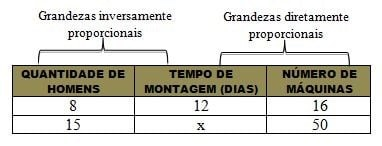
\includegraphics[height=30mm]{assets/R3composta.jpg}
    \end{tabular}

    Analisemos as grandezas a fim de saber se são direta ou inversamente proporcionais entre si.

    Fixando a grandeza quantidade de homens, vamos relacionar as grandezas tempo de montagem com número de máquinas. Se dobrarmos o tempo de montagem, dobraremos o número de máquinas. Logo, essas duas grandezas são diretamente proporcionais.

    Fixando a grandeza número de máquinas, vamos relacionar as grandezas quantidade de homens com tempo de montagem. Se dobrarmos o número de homens, teremos reduzido à metade o tempo de montagem. Logo, essas duas grandezas são inversamente proporcionais.

    Sabendo dessas informações, basta escrevermos a proporção de acordo com a tabela acima;

    Como temos grandezas inversamente proporcionais, devemos inverter uma das frações;

    $ \dfrac{12}{x} = \dfrac{8}{15} \cdot \dfrac{16}{50} \to \dfrac{12}{x} = \dfrac{15}{8} \cdot \dfrac{16}{50}  $\\

    $ \dfrac{12}{x} = \dfrac{240}{400}$

    $ 240x = 12 \cdot 400 \to x = \dfrac{4800}{240} \to x = 20 $ dias. Com 15 homens, construirão 50 máquinas em 20 dias.

    \subsection{Exercícios de Grandezas}

    \begin{enumerate}

        \item (UNCISAL/2019) As equipes M e N classificaram-se para disputar o título anual de um campeonato de voleibol. A equipe campeã, aquela que conseguir 7 vitórias sobre a outra, ganhará R\$ 360.000,00 como prêmio. Devido a problemas estruturais no ginásio em que as partidas aconteciam, a disputa foi encerrada quando a equipe M possuía 6 vitórias e a equipe N, 4 vitórias. Considerando esse placar, as equipes decidiram que a forma mais justa de dividir o prêmio, seria fazê-la de forma proporcional às probabilidades de uma ou outra ser campeã, se as partidas restantes viessem a ser disputadas no “cara ou coroa”.

              Nas condições acordadas entre as equipes, as quantias que M e N, respectivamente, deverão receber são:

              a)	  R$ 270 000,00 e R$ 90 000,00.

              b)	  R$ 324 000,00 e R$ 36 000,00.

              c)	  R$ 216 000,00 e R$ 144 000,00.

              d)	  R$ 315 000,00 e R$ 45 000,00.

              e)	  R$ 240 000,00 e R$ 120 000,00.

        \item (ESPM-SP) Em 10 minutos, 27 secretárias com a mesma habili- dade digitaram o equivalente a 324 páginas.

              Nas mesmas condições, se o número de secretárias fosse 50, em quantos minutos teorica- mente elas digitariam 600 páginas?

              a) 10min

              b) 45min

              c) 5min

              d) 5min e 24seg

              e) 34min e 29seg

        \item (ENEM) Uma escola lançou uma campanha para seus alunos arrecadarem, durante 30 dias, alimentos não perecíveis para doar a uma comunidade carente da região. Vinte alunos aceitaram a tarefa e nos primeiros 10 dias trabalharam 3 horas diárias, arrecadando 12 kg de alimentos por dia. Animados com os resultados, 30 novos alunos somaram-se ao grupo, e passaram a trabalhar 4 horas por dia nos di- as seguintes até o término da campanha. Admitindo-se que o ritmo de coleta tenha se mantido constante, a quantidade de alimentos arrecadados ao final do prazo estipulado seria de:

              a)920kg

              b)800kg

              c)720kg

              d)600kg

              e)570kg

        \item (UFG) Para encher um recipiente de 5 litros, uma torneira gasta 12 se- gundos. Uma segunda torneira gasta 18 segundos para encher o mesmo recipiente. Nestas condições, para encher um tanque de 1000 litros, usando as duas torneiras ao mesmo tempo, serão necessários, em minutos:

              a) $20 \ $ b) $24 \ $ c) $33 \ $ d) $50 \ $ e) $83 $

        \item (Vunesp) Para uma prova, 150 candidatos deveriam ser acomodados nas salas A, B, C e D de um colégio, com capacidade para receber 60, 50, 40 e 30 candidatos, respectivamente. A organização decidiu preencher inicialmente todos os lugares da sala menor, e os candidatos restantes foram repartidos entre as demais salas de forma diretamente proporcional à capacidade de cada uma. O número de lugares não ocupados na sala de maior capacidade foi igual a:

              a) $8 \ $ b) $10 \ $ c) $12 \ $ d) $14 \ $ e) $16 $

        \item (Enem) Fontes alternativas. Há um novo impulso para produzir combustível a partir de gordura animal. Em abril, a High Plains Bioenergy inaugurou uma biorrefinaria próxima a uma fábrica de processamento de carne suína em Guymon, Oklahoma. A refinaria converte a gordura do porco, juntamente com o óleo vegetal, em biodiesel. A expectativa da fábrica é transformar 14 milhões de quilogramas de banha em 112 milhões de litros de biodiesel.

              Revista Scientific American. Brasil, ago. 2009 (adaptado).

              Considere que haja uma proporção direta entre a massa de banha transformada e o volume de biodiesel produzido.

              Para produzir 48 milhões de litros de biodiesel, a massa de banha necessária, em quilogramas, será de, aproximadamente,

              A) 6 milhões.

              B) 33 milhões.

              C) 78 milhões.

              D) 146 milhões.

              E) 384 milhões.

        \item Os ângulos de um triângulo são diretamente proporcionais aos números 3, 7 e 15, então, podemos afirmar que o menor ângulo mede:

              a) 108°  b) 50,4°  c) 21,6°  d) 42°  e) 50,4°

        \item Os lados de um retângulo são proporcionais a 2 e 3. Sabendo que a sua área é de 216 m², as dimensões dos retângulos são, respectivamente:

              A) 12 e 18

              B) 4 e 54

              C) 8 e 27

              D) 10 e 26

              E) 13,5 e 16

        \item Uma herança de R\$ 1.500.000 foi dividida entre os filhos de forma diretamente proporcional à idade de cada um deles. Sabendo que há três filhos, com 14, 16 e 20 anos de idade, podemos afirmar que o filho do meio receberá:

              A) R\$ 600.000

              B) R\$ 420.000

              C) R\$ 480.000

              D) R\$ 500.000

              E) R\$ 450.000

        \item Os ângulos de um quadrilátero são proporcionais a 3, 6, 12, 15. Assim, podemos afirmar que o valor do maior ângulo é:

              .a) 150°  .b) 120°  .c) 60°  .d) 30°  .e) 135°

        \item A idade de três irmãos é diretamente proporcional a 4, 6 e 10 anos. Sabendo que a soma da idade dos três é igual a 70, podemos afirmar que o mais novo possui:

              A) 10 anos

              B) 12 anos

              C) 14 anos

              D) 16 anos

              E) 18 anos

        \item Um automóvel faz 35 km com 5 litros de etanol. Realizando uma viagem de uma cidade para outra, com base nesse consumo, qual deve ser a quantidade de etanol necessária para percorrer 170 km?

              A) 28 litros

              B) 25 litros

              C) 20 litros

              D) 30 litros

              E) 18 litros

        \item Das relações entre as grandezas a seguir, identifique aquela que não é diretamente proporcional.

              A) Quantidade de funcionários e produtividade

              B) Distância percorrida e consumo do veículo

              C) Velocidade do automóvel e tempo para completar o percurso

              D) Valor pago pela verdura e peso

        \item Um triângulo retângulo possui os lados diretamente proporcionais a 3, 4 e 5. Sabendo que sua hipotenusa é igual a 31 cm, o valor do perímetro desse triângulo é:

              A) 28,4 cm

              B) 42,6 cm

              C) 65 cm

              D) 74,4 cm

              E) 82,8 cm

    \end{enumerate}

    \section*{P.A. e P.G.}

    \subsection{Progressão Aritmética P.A.}

    A Progressão Aritmética (P.A.) é uma sequência de números onde a diferença entre dois termos consecutivos é sempre a mesma. Essa diferença constante é chamada de razão da P.A..

    Sendo assim, a partir do segundo elemento da sequência, os números que surgem são resultantes da soma da constante com o valor do elemento anterior.

    Isso é o que a diferencia da progressão geométrica (P.G.), pois nesta, os números são multiplicados pela razão, enquanto na progressão aritmética, eles são somados.

    As progressões aritméticas podem apresentar um número determinado de termos (P.A. finita) ou um número infinito de termos (P.A. infinita).

    Para indicar que uma sequência continua indefinidamente utilizamos reticências, por exemplo:

    A sequência (4, 7, 10, 13, 16, ...) é uma P.A. infinita.

    A sequência (70, 60, 50, 40, 30, 20, 10) é uma P.A. finita.

    Cada termo de uma P.A. é identificado pela posição que ocupa na sequência e para representar cada termo utilizamos uma letra (normalmente a letra "a") seguida de um número que indica sua posição na sequência.

    Por exemplo, o termo a4 na P.A (2, 4, 6, 8, 10) é o número 8, pois é o número que ocupa a 4ª posição na sequência.

    \textbf{Classificação de uma P.A.}

    De acordo com o valor da razão, as progressões aritméticas são classificadas em:

    \textbf{Constante:} quando a razão for igual a zero. Por exemplo: (4, 4, 4, 4, 4...), sendo r = 0.

    \textbf{Crescente:} quando a razão for maior que zero. Por exemplo: (2, 4, 6, 8,10...), sendo r = 2.

    \textbf{Decrescente:} quando a razão for menor que zero (15, 10, 5, 0, - 5,...), sendo r = - 5

    \textbf{Propriedades da P.A.}

    \textbf{1ª Propriedade:}

    Em uma P.A. finita, a soma de dois termos equidistantes dos extremos é igual à soma dos extremos.

    \begin{tabular}{@{}c@{}}
        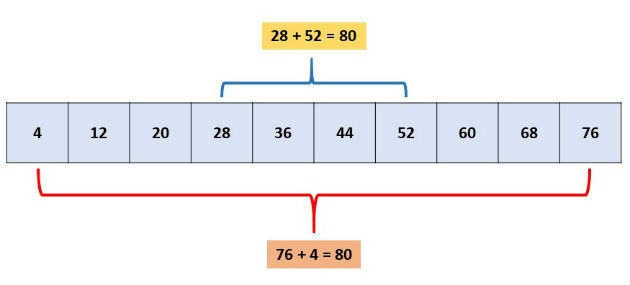
\includegraphics[height=30mm]{assets/papropriedade1.jpg}
    \end{tabular}

    \textbf{2ª Propriedade}

    Considerando três termos consecutivos de uma P.A., o termo do meio será igual a média aritmética dos outros dois termos.

    \begin{tabular}{@{}c@{}}
        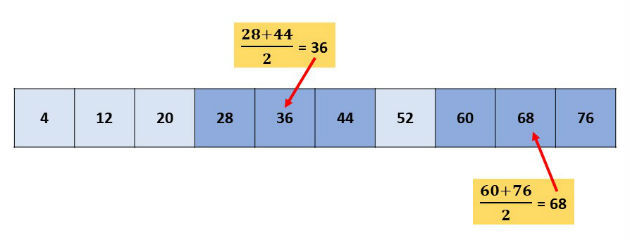
\includegraphics[height=30mm]{assets/papropriedade2.jpg}
    \end{tabular}

    \textbf{3ª Propriedade}

    Em uma P.A. finita com número de termos ímpar, o termo central será igual a média aritmética entre termos equidistantes deste. Esta propriedade deriva da primeira.

    \begin{tabular}{@{}c@{}}
        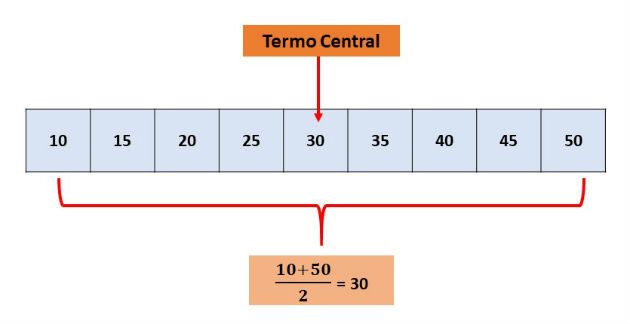
\includegraphics[height=30mm]{assets/papropriedade3.jpg}
    \end{tabular}

    \textbf{Fórmula do Termo Geral de uma P.A.}

    $ an = a_1 + (n - 1) \cdot r $

    Onde,

    \textbf{an:} termo que queremos calcular

    \textbf{a1:} primeiro termo da P.A.

    \textbf{n:} posição do termo que queremos descobrir

    \textbf{r:} razão

    \textbf{Explicação da fórmula}:

    Como a razão de uma P.A. é constante, podemos calcular seu valor a partir de quaisquer termos consecutivos, ou seja:

    $ r = a_2 - a_1 = a_3 - a_2 = a_4 - a_3 = a_5 - a_4 = a_6 - a_5 \, \cdots \, a_n - a_{n-1} $

    Sendo assim, podemos encontrar o valor do segundo termo da P.A. fazendo:

    $ a_2 - a_1 = r  \to a_2 = a_1 + r $

    Para encontrar o terceiro termo utilizaremos o mesmo cálculo:

    $ a_3 - a_2 = r  \to a_3 = a_2 + r $

    Substituindo o valor de $a_2$, que encontramos anteriormente, temos:

    $ a_3 = (a_1 + r) + r \ \ \ \to \ \ \ a_3 = a_1 + 2r $

    Se seguirmos o mesmo raciocínio, podemos encontrar:

    $ a_4 - a_3 = r \ \ \to \ \ a_4 = a_3 + r \ \ \to \ \ a_4 = a_1 + 3r $

    Observando os resultados encontrados, notamos que cada termo será igual a soma do primeiro termo com a razão multiplicada pela posição anterior.

    Esse cálculo é expresso através da fórmula do termo geral da P.A., que nos permite conhecer qualquer elemento de uma progressão aritmética.

    \textbf{Exemplo:}

    Calcule o 13° termo da P.A.: ( 26, 31, 36, 41, 46, 51...). Temos:

    $ \ \ a_1 = 26 \ \ \to \ \ r = 31 - 26 = 5 \ \ \to \ \ n = 13 \ (13^0 \ termo)$.

    Substituindo os valores na fórmula, temos:

    $ a_n = a_1 + (n - 1) \cdot r $.

    $ a_{13} = 26 + (13 - 1) \cdot 5 $

    $ a_{13} = 26 + 12 \cdot 5 $

    $ a_{10} = 86 $

    \textbf{Fórmula do termo geral para um k qualquer}.

    Para definir um termo aleatório qualquer, que chamamos de an, não temos o primeiro termo a1, mas conhecemos outro qualquer, que chamamos de ak.

    Podemos usar a fórmula do termo geral a partir de um termo k qualquer:

    $ a_n = a_k + (n - k) \cdot r $

    Repare que a única diferença, foi a mudança do índice 1 na primeira fórmula, pelo k, na segunda. Sendo:

    an: o n-ésimo termo da P.A. (um termo numa posição n qualquer)
    ak: o k-ésimo termo de uma P.A. (um termo numa posição k qualquer)
    r: a razão

    \textbf{Soma dos termos de uma P.A.}

    Para somar os termos de uma P.A. finita, devemos usar a seguinte fórmula:

    $ S_n = \dfrac{(a_1 + a_n) \cdot n}{2} \ \ \ \ \ $	, onde:

    \textbf{Sn:} soma dos n primeiros termos da P.A.
    \textbf{a1:} primeiro termo da P.A.
    \textbf{an:} ocupa a enésima posição na sequência (uma termo na posição n)
    \textbf{n:} posição do termo.

    \subsection{Exercícios de P.A.}

    \begin{enumerate}

        \item PUC/RJ - 2018 Sabendo que os números da sequência (y, 7, z, 15) estão em progressão aritmética, quanto vale a soma y + z?

              a) $20 \ $ b) $14 \ $ c) $7 \ $ d) $3,5 \ $ e) $2 $

        \item O preço de uma máquina nova é R\$ 150 000,00. Com o uso, seu valor sofre uma redução de R\$ 2 500,00 por ano. Sendo assim, por qual valor o proprietário da máquina poderá vendê-la daqui a 10 anos?

        \item Um ciclista percorre 15 km na primeira hora de uma corrida. Na segunda hora de corrida, seu rendimento cai e ele só consegue percorrer 13 km, e na hora seguinte 11 km. Continuando nesta sequência, quantos quilômetros ele conseguirá percorrer nas 6 horas de prova?

        \item Unicamp - 2015

              Se (a1, a2,..., a13) é uma progressão aritmética (PA) cuja soma dos termos é igual a 78, então a7 é igual a

              a) $6 \ $ b) $7 \ $ c) $8 \ $ d) $9 $

        \item Fuvest - 2012 Considere uma progressão aritmética cujos três primeiros termos são dados por $ a_1 = 1 + x, a_2 = 6x, a_3 = 2x^2 + 4$, em que x é um número real.

              a) Determine os possíveis valores de x.
              b) Calcule a soma dos 100 primeiros termos da progressão aritmética correspondente ao menor valor de x encontrado no item a)

        \item AFA - Em um pentágono, os ângulos internos estão em Progressão Aritmética. Qual o terceiro termo, em graus, dessa progressão?

              a) $54 \ $ b) $108 \ $ c) $162 \ $ d) $216 $

    \end{enumerate}

    \subsection{Progressão Geométrica P.G.}

    \textbf{P.G. ou Progressão Geométrica} é uma sequência numérica onde os termos a partir do segundo termo são obtidos multiplicados por uma constante "\textbf{q}" a qual chamamos razão.

    Para encontrarmos a razão de uma P.G., basta dividirmos um número pelo seu antecessor.

    \textbf{Tipos de Progressão Geométrica}

    \textbf{Crescente}: Onde cada termo da P.G. é maior que o seu antecessor.

    $ -4, -2, -1, \frac{1}{2}, \frac{1}{4} $ com q = 2;

    $ \{ 2, 4, 8, 16, 32 \} $ P.G. crescente de razão q = 2.

    \textbf{Decrescente}: Onde cada termo da P.G. é menor que o seu antecessor.

    $ 4, 2, 1, \frac{1}{2}, \frac{1}{4}, \frac{1}{8} $ com q = $\frac{1}{2}$;

    $ \{ 270, 90, 30, 10, \frac{10}{3}\} $ P.G. decrescente de razão q = 3.

    \textbf{Constante}: Onde cada termo da P.G. é sempre igual. Isso acontece quando a razão q = 1.

    $\{ 5, 5, 5, 5, 5 \}$;

    $\{ 7, 7, 7, 7,7 \}$.

    \textbf{Oscilante}: É quando os valores se alternam entre positivo e negativo. Isso acontece quando o valor da razão é um número negativo, q = -2 por exemplo.

    $ \{ 3, -9, 27, -81, 243 \}$ Oscilante com razão q = $-3$;

    $ \{ 5, -25, 125, -625 \}$ Oscilante com razão q = $-5$.

    \textbf{Fórmula do Termo Geral de uma P.G.}

    Para encontrar qualquer elemento da P.G., utiliza-se a expressão:

    $ a_n = a_1 \cdot q^{n -1} $.

    Onde:

    an: número que queremos obter;

    a1: o primeiro número da sequência;

    q(n-1): razão elevada ao número que queremos obter, menos 1.

    Assim, para identificar o termo 20 de uma P.G. de razão q = 2 e número inicial 2, calcula-se:

    PG: (2,4,8,16, 32, 64, 128,...)

    $ a_20 = 2 . 2^{20-1} $;

    $ a_20 = 2 . 2^{19} $;

    $ a_20 = 1.048.576 $.

    \textbf{Soma dos Termos da P.G.}

    Para calcular a soma dos números presentes numa P.G., utiliza-se a seguinte fórmula:

    $ S_n = \dfrac{a_1 \cdot (q^{n -1})}{q -1} $, onde:

    \textbf{Sn}: Soma dos números da P.G.;

    \textbf{a1}: primeiro termo da sequência;

    \textbf{q}: razão;

    \textbf{n}: quantidade de elementos da P.G..

    Dessa forma, para calcular a soma dos 10 primeiros termos da seguinte P.G. (1,2,4,8,16, 32,...):

    $ S_n = \dfrac{a_1 \cdot (q^{n -1})}{q -1} $;

    $ S_{10} = \dfrac{1 \cdot (2^{10 -1})}{2 -1} $;\\

    $ S_{10} = \dfrac{1024 -1}{1} \ \ \ \ \ \to \ \ \ \ \ = 1023 $.

    \textbf{Observação:} Na P.A. nós somamos a razão ao termo seguinte, e na P.G. nós multiplicamos pela razão o termo seguinte.

    \subsection{Exercícios de P.G.}

    \begin{enumerate}

        \item  (FUVEST) – Numa progressão geométrica de quatro termos positivos, a soma dos dois primeiros vale 1 e a soma dos dois últimos vale 9. calcule a razão da progressão.

              a) $3 \ \ \ $ b) $5 \ \ \ $ c) $7 \ \ \ $ d) $9 \ \ \ $ e) $11$

        \item (UE – PA) – Um carro, cujo preço à vista é R\$ 24 000,00, pode ser adquirido dando-se uma entrada e o restante em 5 parcelas que se encontram em progressão geométrica. Um cliente que optou por esse plano, ao pagar a entrada, foi informado que a segunda parcela seria de R\$ 4 000,00 e a quarta parcela de R\$ 1 000,00. Quanto esse cliente pagou de entrada na aquisição desse carro?

              a) R\$ 7 500,00 $ \ $ b) R\$ 8 500,00

              c) R\$ 8 550,00 $ \ $ d) R\$ 7 550,00

              e) R\$ 5 800,00

        \item  (PUC-RIO 2008) – Na seqüência (1, 3, 7,…), cada termo é duas vezes o anterior mais um. Assim, por exemplo, o quarto termo é igual a 15. Então o décimo termo é:

              a) $1000 \ \ $ b) $1002 \ \ $ c) $1015 \ \ $

              d) $1023 \ \ $ e) $1024 $

        \item (UDESC 2010) – Os termos (a, b, c) formam, nesta ordem, uma progressão aritmética crescente, cuja soma é igual a 21.

              Então os termos formam, nesta ordem, uma progressão geométrica de razão igual a:

              a) $-2 \ $ b) $2 \ $ c) $16 \ $ d) $4 \ $ e) $-4$

        \item (FIA) – Numa progressão geométrica, tem-se a3 = 40 e a6 = -320. A soma dos oito primeiros termos é:

              a) $-1700 \ \ $ b) $-850 \ \ $ c) $850 \ \ $

              d) $1700 \ \ \ \ $ e) $750 $

        \item CESGRANRIO, 1991) Um artigo custa hoje R\$ 100,00 e seu preço é aumentado, mensalmente, em 12\% sobre o preço anterior. Se fizermos uma tabela do preço desse artigo mês a mês, obteremos uma Progressão

              a) Aritmética de razão 12.

              b) Aritmética de razão 0,12.

              c) Geométrica de razão 12.

              d) Geométrica de razão 1,12.

              e) Geométrica de razão 0,12.

        \item (UDESC, 2011) Em uma escola com 512 alunos, um aluno apareceu com o vírus do sarampo. Se esse aluno permanecesse na escola, o vírus se propagaria da seguinte forma: no primeiro dia, um aluno estaria contaminado; no segundo, dois estariam contaminados; no terceiro, quatro, e assim sucessivamente. A diretora dispensou o aluno contaminado imediatamente, pois concluiu que todos os 512 alunos teriam sarampo no:

              a) $9^0 \ \ $ b) $10^0 \ \ $ c) $8^0 \ \ $

              d) $5^0 \ \ $ e) $6^0 $

        \item (UFSM, 2008) Uma fábrica vendia 12 camisetas por mês para certa rede de academias desde janeiro de um determinado ano. Devido ao verão, essa venda foi triplicada a cada mês, de setembro a dezembro. O total de camisetas vendidas nesse quadrimestre e a média de vendas, por mês, durante o ano, foram, respectivamente,

              a) 1.536 e 128

              b) 1.440 e 128

              c) 1.440 e 84

              d) 480 e 84

              e) 480 e 48



    \end{enumerate}



    \section*{Representação e Análise de Dados}

    \textbf{ Estatística é uma Ciência} que se aplica em todos os campos do conhecimento. Costuma-se dizer que é a ciência que trata dos dados. Os dados têm sido, desde há muitos séculos, instrumentos essenciais à compreensão do mundo que nos rodeia. Neste capítulo procedemos à classificação dos dados, processo este que condiciona, de um modo geral, a ferramenta estatística a utilizar na sua organização e no seu tratamento.

    A Estatística é bastante utilizada em diversos ramos da sociedade, no intuito de realizar pesquisas, colher dados e processá-los, analisar informações, apresentar situações através de gráficos de fácil compreensão. Os meios de comunicação, ao utilizarem gráficos, deixam a leitura mais agradável. O IBGE (Instituto Brasileiro de Geografia e Estatística) é considerado um órgão importante e conceituado na área. No intuito de conhecer e aprofundar nos estudos estatísticos precisamos conhecer alguns conceitos e fundamentos primordiais para o desenvolvimento de uma pesquisa.

    \textbf{Conceitos e Fundamentos}

    \textbf{População}: conjunto de elementos, número de pessoas de uma cidade.

    \textbf{Amostra}: parte representativa de uma população.

    \textbf{Variável}: depende da abordagem da pesquisa, da pergunta que será feita. Exemplo: Qual sua marca de carro favorita? Ford, Volks, Fiat, Peugeot, Nissan são alguns exemplos de resposta.

    \textbf{Frequência absoluta}: valor exato, número de vezes que o valor da variável é citado.

    \textbf{Frequência relativa}: valor representado através de porcentagem, divisão entre a frequência absoluta de cada variável e o somatório das frequências absolutas.

    \textbf{Medidas de tendência central}

    \textbf{Média aritmética}: medida de tendência central. Somatório dos valores dos elementos, dividido pelo número de elementos.

    \textbf{Média aritmética ponderada}: Somatório dos valores dos elementos multiplicado pelos seus respectivos pesos, dividido pela soma dos pesos atribuídos.

    \textbf{Moda}: valor de maior frequência em uma série de dados, o que mais se repete.

    \textbf{Mediana}: medida central em uma determinada sequência de dados numéricos.

    \textbf{Medidas de dispersão}

    \textbf{Amplitude}: subtração entre o maior valor e o menor valor dos elementos do conjunto.

    \textbf{Variância}: dispersão dos dados variáveis em relação à média.

    \textbf{Desvio Padrão}: raiz quadrada da variância. Indica a distância média entre a variável e a média aritmética da amostra.








    %1	 operações em conjuntos numéricos		
    %2	 porcentagem e juros		
    %3	 principio de contagem		
    %4	 razão e proporção		
    %5	 relações de dependência entre grandezas		
    %6 	 sequências de progressão		PA e PG
    %7	 representação e análise de dados		
    %8	 Noções básicas de estatística e probabilidade		
    %9	 medidas de tendência central		
    %10 medidas de posição		
    %11	 desvios e variância		
    %12 noções de probabilidade	






\end{multicols*}